\chapter{Cosmologia}
\label{cha:cosmologia}

\section{Equazioni di Einstein: Modello di Friedmann}

Si assume che la dinamica dell'Universo sia governata dalle eq. di Einstein, che
la metrica sia quella di RW e che il tensore energia-impulso sia quello di un
fluido perfetto.  La metrica dello spazio-tempo è
\begin{subequations}
  \label{rw1}
  \begin{align}
    g_{tt} &=-1, \\
    g_{it} &= 0, \\
    g_{ij} &= R^2(t) \tilde{g}_{ij}(x^i),
  \end{align}
\end{subequations}
dove $t$ è il tempo cosmico, $x^{i} = (r,\theta,\phi)$ sono coordinate sferiche
coomoventi e $\tilde{g}_{ij}(x^i)$ è la metrica su $^{3}$S
\begin{subequations}
  \label{rw2}
  \begin{align}
    \tilde{g}_{rr} &= (1-kr^2)^{-1}, \\
    \tilde{g}_{\theta \theta} &= r^2, \\
    \tilde{g}_{\phi \phi} &= r^2 \sin^2 \phi,
  \end{align}
\end{subequations}
tutti gli altri elementi della metrica sono nulli.

Il tensore energia-impulso ha la forma
\begin{equation}
  T_{\mu\nu} = p g_{\mu\nu} + (p+\rho) U_{\mu} U_{\nu}
  \label{fp}
\end{equation}
con $p$ pressione, $\rho$ densità di energia e $U^{\mu}=(1,0,0,0)$ 4-velocità
dei costituenti dell'Universo.

La dinamica dell'Universo è determinata dalle eq. di Einstein
\begin{equation}
  R_{\mu\nu} =-8\pi GS_{\mu \nu},
\end{equation}
con
\begin{equation}
  S_{\mu \nu}=T_{\mu \nu}-\frac{1}{2} g_{\mu \nu} \tensor{T}{^{\lambda}_{\lambda}}.
\end{equation}

Il tensore di Ricci diventa (il punto indica derivazione rispetto al tempo)
\begin{subequations}
  \begin{align}
    R_{tt} &= \frac{ 3 \ddot{R}}{R} \\
    R_{ti} &= 0 \\
    R_{ij} &= -(R\ddot{R}+2\dot{R}^2+2k) \tilde{g}_{ij}.
  \end{align}
\end{subequations}

Osserva che
\begin{equation}
  \tensor{T}{^{\lambda}}{_{\lambda}} = g^{\lambda\nu} T_{\lambda\nu} = p
  \tensor{\delta}{^{\lambda}}_{{\lambda}} + (p+\rho) (-1) = 3p - \rho
\end{equation}
così che il termine di sorgente diventa
\begin{equation}
  S_{\mu \nu} = \frac{1}{2} (\rho-p) g_{\mu\nu}+(p+\rho)U_{\mu} U_{\nu}
\end{equation}
In particolare
\begin{subequations}
  \begin{align}
    S_{tt} &= \frac{1}{2} (\rho-p)(-1)+(p+\rho)(+1) =
             \frac{1}{2} (\rho+3p) \\
    \label{sij}
    S_{ij} &= \frac{1}{2} (\rho-p) g_{ij}=
             \frac{1}{2} (\rho-p) R^2(t) \tilde{g}_{ij}
  \end{align}
\end{subequations}

Dalle eq. di Einstein per la componente $tt$ si ha:
\begin{equation}
  \frac{3 \ddot{R}}{R} = - 4\pi G (\rho+3p)
  \label{e1}
\end{equation}
e per la componente $ij$:
\begin{equation}
  \label{e2}
  \frac{\ddot{R}}{R} +\frac{2\dot{R}^2}{R^2}+\frac{2k}{R^2}= 4 \pi G (\rho-p)
\end{equation}
Si ha inoltre l'eq. di conservazione (da $\tensor{T}{^{\mu \nu}_{;\mu}}=0$, con $\nu =0$)
\begin{equation}
  \dot{p} R^3 = \toder{}{t}[R^3(\rho+p)]  \iff \toder{(\rho R^3)}{R} = -3pR^2
  \label{moto}
\end{equation}

Si osservi che le tre eq.  \eqref{e1}, \eqref{e2} e \eqref{moto} non sono
indipendenti (una può essere derivata dalle altre due).  Pertanto per risolvere
il problema cosmologico, cioè per determinare $R$, $\rho$ e $p$ in funzione del
tempo cosmico, è necessario introdurre un'ulteriore relazione.  Questa è
l'eq. di stato
\begin{equation}
  p=p(\rho)
  \label{stato}
\end{equation}
che ha i casi particolari $p=0$ per l'era della materia, $p=\rho/3$ per l'era
della radiazione.

Osserviamo infine che eliminando $\ddot{R}$ tra le eq.  \eqref{e1} e \eqref{e2},
si ottiene un'equazione differenziale del primo ordine, nota come
\emph{equazione di Friedmann}
\begin{equation}
  \dot{R}^2 +k = \frac{8 \pi G}{3} \rho R^2.
  \label{eq:friedmann}
\end{equation}

In conclusione, le eq. \eqref{eq:friedmann}, \eqref{moto} e \eqref{stato}
permettono di determinare le 3 funzioni incognite $R(t)$, $p(t)$ e $\rho(t)$.
Si otterranno 3 differenti soluzioni a seconda del valore di $k=-1,0,+1$.
Questi modelli cosmologici sono noti come modelli di Friedmann.

\textbf{Osservazione}: senza dare esplicitamente l'eq. di stato è possibile
ricavare informazioni sull'età $t_0$ dell'Universo e sull'andamento del fattore
di scala cosmico $R(t)$.  Infatti:
\begin{itemize}
\item $R(t)$ è una quantità definita positiva;
\item All'istante attuale $t_0$ l'Universo è in espansione ($\dot{R}_0 >0$)
  poichè noi oggi misuriamo red-shift ($z>0$);
\item L'eq. \eqref{e1} mostra che per materia ordinaria e radiazione $ \ddot{R}
  < 0$ sempre.  Quindi $R(t)$ ha concavità rivolta verso il basso ad ogni tempo,
  il che implica che per $t\rightarrow 0$, necessariamente $R \rightarrow 0$.
  Quindi i modelli di Friedmann prevedono l'esistenza di una singolarità
  iniziale.  Inoltre poichè $ \ddot{R} < 0$ sempre, $\dot{R}$ è una funzione
  decrescente e quindi la velocità di espansione dell'Universo $v_H(t) \propto
  \dot{R}$ diminuisce nel tempo, come ci si aspetta con gravità attrattiva.
\item Il termine a destra nell'eq. \eqref{eq:friedmann}, per $t>t_0$ ($t<t_0$)
  decresce (cresce) con il tempo --- rispetto al valore attuale --- almeno come
  $R^{-1}(t)$.
\end{itemize}

Da queste considerazioni segue che l'età dell'Universo è
\begin{equation}
  t_0 < H^{-1}_0  = \frac {R_0}{\dot{R}_0} = 13 \times 10^{9}
  \left(\frac{\SI[per-mode=reciprocal]{75}{\kilo\metre\per\second\per\mega\parsec}}{H_0}\right)
  \si{yr}.
\end{equation}
L'uguaglianza si avrebbe nel caso in cui fosse $\ddot{R} =0$, per cui $R(t)=t
\dot{R}$.  Per quanto riguarda il comportamento di $R(t)$ per $t>t_0$,
dall'eq. \eqref{eq:friedmann} si ha
\begin{itemize}
\item $R(t) \propto t$ nel caso $k=-1$, per il quale per $t \to \infty$,
  $\dot{R} \to 1$;
\item $R(t) \propto t^{2/3}$ nel caso $k=0$, per il quale per $t \to \infty$,
  $\dot{R} \propto R^{-1/2}$;
\item se $k=-1$, $\dot{R}$ decresce dal valore attuale (positivo) ed esisterà un
  istante $\tilde{t}$ a cui ${\dot R}=0$; a tempi successivi, il fattore di
  scala che ha concavità rivolta sempre verso il basso, continuerà a decrescere
  con il tempo fino ad un nuova singolarità.
\end{itemize}

\subsection{Derivazione newtoniana delle eq. di Friedmann}

Il teorema di Birkhoff afferma che un campo gravitazionale a simmetria sferica è
necessariamente statico ed è descritto dalla metrica di Schwarzschild.  Questo
risultato è l'analogo del risultato newtoniano (derivato dal teorema di Gauss)
che il campo all'esterno di una corpo a simmetria sferica è lo stesso che si
avrebbe se tutta la massa del corpo fosse concentrata al centro.  Il teorema di
Birkhoff può essere applicato anche al campo all'interno di una cavità sferica e
vuota che si trovi al centro di una distribuzione omogenea, non necessariamente
statica, di massa-energia.  In questo caso si prova che la metrica all'interno
della cavità è quella di Minkowski dello spazio piatto (cioè, il campo
gravitazionale è nullo all'interno).  L'analogo newtoniano di questa proprietà è
che il campo gravitazionale all'interno di una shell sferica e vuota è nullo.
Questo risultato è vero anche nel caso in cui la distribuzione di materia sia
infinita, l'unica condizione è che la distribuzione sia sfericamente simmetrica.

Consideriamo una cavità sferica di raggio $l$ al centro di una distribuzione
omogenea di massa.  All'interno la metrica è piatta e il campo gravitazionale è
nullo.  Si rimetta ora nella cavità una quantità di massa $m$, scelta in modo
tale che continui a valere la meccanica newtoniana, cioè
\begin{equation}
  \frac{Gm}{l c^2} \ll 1 \iff l \gg r_g(m).
  \label{41}
\end{equation}
La distanza $l$ nell'Universo in espansione è la distanza propria
\begin{equation}
  l(t) = R(t) r_0
\end{equation}
dove $r_0$ è una coordinata comovente che può essere scelta in modo che sia
valida la condizione in eq. \eqref{41}.  Applichiamo l'approssimazione
newtoniana per descrivere il moto di un punto P sulla sfera di raggio $l(t)$.
Si ha
\begin{equation}
  \toder[2]{l}{t} = -\frac{G m}{l^2} = \frac{4 \pi}{3} G \rho l
  \label{1103}
\end{equation}
o anche, moltiplicando per $\dot l$
\begin{equation}
  \frac{l}{2} \toder{\dot{l}^2}{t} = - \dot{l} \frac{G m}{l^2} = Gm  \toder{}{t}
  \left( \frac{1}{l} \right)
\end{equation}
e integrando
\begin{equation}
  \dot{l}^2 = \frac{2G m}{l} + \text{costante}.
  \label{219}
\end{equation}
Questa eq. rappresenta la conservazione dell'energia per unità di massa.
Utilizzando la relazione $l(t)=R(t) r_0$ si ha
\begin{equation}
  r_0^2 \dot{R}^2 = \frac{2Gm}{r_0 R} - k c^2 r_0^2
  \implies \dot{R}^2 = \frac{2G}{r_0^3 R} \frac{4 \pi \rho R^3 r_0^3}{3} - k c^2
\end{equation}
in cui abbiamo posto $\text{costante} = - k c^2 r_0^2$, con $k=-1$, $0$, $+1$, a
seconda del segno della costante.  Si ha quindi
\begin{equation}
  \dot{R}^2 + k c^2 = \frac{8 \pi}{3} G \rho R^2
  \label{1106}
\end{equation}
che è l'eq. di Friedmann \eqref{eq:friedmann}.  Il caso $k=1$ corrisponde a
$\text{costante}<0$ (energia totale negativa) e quindi il caso descrive la
situazione in cui un'eventuale espansione è seguita da collasso; il caso $k=-1$
corrisponde a $\text{costante}>0$ (energia totale positiva) e quindi espansione
continua per sempre.  Il caso $k=0$ corrisponde ad energia totale nulla e
rappresenta la situazione limite con velocità di espansione pari alla velocità
di fuga, per cui l'espansione cessa solamente per $t\to \infty$.

L'eq. \eqref{1106} è stata ottenuta assumendo che la sfera di raggio $l$
contenga solo materia non relativistica.  In Relatività Generale in presenza di
materia relativistica si ha che la densità di materia deve essere rimpiazzata da
(vedi eq. \eqref{e1})
\begin{equation}
  \rho \to  \rho + \frac{3 p}{c^2}
\end{equation}
dove $\rho$ è ora l'energia totale (energia associata alla massa a riposo +
energia interna).  In questo modo l'eq. \eqref{1103} diventa
\begin{equation}
  \ddot R = - \frac{4 \pi G }{3} \left( \rho + 3 \frac{p}{c^2} \right) R,
\end{equation}
che è l'analoga eq. \eqref{e1} ottenuta applicando la Relatività Generale.

Per quanto riguarda l'eq. di conservazione \eqref{moto}, essa si può ottenere
dalla I legge della termodinamica nel caso di espansione dell'Universo
adiabatica ($\dd Q=0$).  Si ha
\begin{equation}
  \dd U + p \dd V=0
\end{equation}
e sostituendo $U=\rho V c^2$, per cui $\dd U= V c^2 d\rho + \rho c^2 \dd V$, si
ha
\begin{equation}
  \rho \dd V + V \dd\rho = - \frac{p}{c^2} \dd V \implies
  \dd\rho= -\left( \rho + \frac{p}{c^2} \right) \frac{\dd V}{V}
\end{equation}
da cui segue
\begin{equation}
  \label{eq:continuita}
  d\rho= - \left( \rho + \frac{p}{c^2} \right) \frac{4 \pi l^2 dl}{4 \pi l^3/3}
  \implies \toder{\rho}{t} +  3 \left( \rho + \frac{p}{c^2} \right) \frac{\dot
    R }{R} =0
\end{equation}
che è equivalente all'eq. \eqref{moto}.

La densità critica $\rho_c$ si può ottenere ponendo in eq. \eqref{219}
$v=v_{c}$.  Si ha
\begin{equation}
  v^2_{c} = \frac{2 G m }{l}=\frac{2G}{l} \frac{4}{3} \pi \rho_c l^3 \implies
  \dot{R}^2= \frac{8 \pi G}{3} \rho_c R^2
\end{equation}
e per l'istante attuale $t_0$
\begin{equation}
\rho_c(t_{0}) = \frac{3 H_0^2}{8 \pi G}.
\end{equation}

\section{Densità e pressione dell'Universo presente}

All'istante attuale densità e pressione sono valutate dalle eq. dinamiche (con $t=t_0$)
\begin{subequations}
  \begin{align}
    \label{rho0}
    \rho_0  &= \frac{3}{8 \pi G} \left(\frac{k}{R_0^2} + H_0^2 \right) \\
    \label{p0}
    p_0 &= -\frac{1}{8 \pi G} \left[\frac {k}{R_0^2}+H_0^2(1-2q_0)\right].
  \end{align}
\end{subequations}
Se si definisce una \emph{densità critica}
\begin{equation}
  \rho_c \equiv  \frac{3 H_0^2}{8 \pi G} = 1.1 \times 10^{-29}
  \left(
    \frac{H_0}{\SI[per-mode=reciprocal]{75}{\kilo\metre \per \second \per
        \mega\parsec}}
  \right)^2
  \si{\gram\per\centi\metre\cubed}
  \label{rhoc}
\end{equation}
l'eq. \eqref{rho0} diventa
\begin{equation}
  \rho_0-\rho_c =  \frac{3 k}{8 \pi G R_0^2},
  \label{temp1}
\end{equation}
per cui l'Universo ha curvatura spaziale positiva o negativa a seconda che sia
$\rho_0 > \rho_c$ oppure $\rho_0 < \rho_c$.

Possiamo mettere in relazione $\rho_0$ e $\rho_c$ con il parametro di
decelerazione $q_0$.  Infatti per l'Universo presente che è dominato dalla
materia, si ha $p_0=0$, così che dall'equazione~\eqref{p0} segue
\begin{equation}
  \frac{k}{R_0^2} = H_0^2 (2q_0-1)
\end{equation}.
Sostituendo nella \eqref{temp1} si ottiene infine
\begin{equation}
  \frac{\rho_0}{\rho_c}=2 q_0
  \label{rho0surhoc}
\end{equation}
pertanto
\begin{itemize}
\item se $q_0 > 1/2 \implies \rho_0>\rho_c$, $k=+1$
\item se $q_0 = 1/2 \implies \rho_0=\rho_c$, $k=0$
\item se $q_0 < 1/2 \implies \rho_0<\rho_c$, $k=-1$
\end{itemize}

Poiché oggi $\rho_*(0) \ll \rho_c$ e inoltre la radiazione di fondo cosmico non
contribuisce in maniera apprezzabile a $\rho_0$, se $q_0 \ge 0.5$ esisterà
nell'Universo DM.  La densità di energia mancante non potrà comunque essere in
forma di barioni (diffusi sotto forma di idrogeno neutro e/o molecolare) poiché
per la Nucleosintesi (come si vedrà) $\rho_B < 0.05 \rho_c$.

\section{Era dominata dalla materia}

All'istante attuale l'Universo è nell'era della materia, e questa si estende
indietro nel tempo fino a valori di red-shift $z \simeq 1000$.  Infatti dalla
relazione
\begin{equation}
  \frac {\rho_m(t)} {\rho_r(t)} \simeq  10^{3} \frac {R(t)} {R_0} \equiv  10^3
  \frac{1}{1+z}
\end{equation}
si ha che l'Universo entra nell'era della radiazione ($\rho_m = \rho_r$) quando
$z = 1000$.  Questo accade (come vedremo) ad un tempo $ \simeq 10^5$ yr (a
partire dalla singolarità iniziale).  Tale valore è trascurabile rispetto al
tempo attuale dell'Universo $t_0 \simeq 14 \times 10^9$ yr e pertanto porremo
l'inizio di tale era a $t=0$.  Riprendiamo in esame l'eq. di Friedmann
\eqref{eq:friedmann} in cui poniamo
\begin{equation}
  \rho = \rho_0 \left( \frac {R_0} {R} \right)^{3}
\end{equation}
È conveniente esprimere $\rho_0$ e $k/R^2$ in termini di $q_0$ ed $H_0$.
Dall'eq. \eqref{p0} segue
\begin{equation}
  \frac{k}{R_0^2}=(2q_0-1) H_0^2~,
\end{equation}
e sostituendo nell'eq. \eqref{rho0} si ha
\begin{equation}
  \frac{8\pi G}{3} \rho_0 = 2q_0 H_0^2
\end{equation}
Usando le relazioni precedenti l'eq. \eqref{eq:friedmann} diventa:
\begin{equation}
  \dot{R}^2 + (2 q_0-1) H_0^2 R_0^2 = \frac{8\pi G}{3} \rho_0 \frac{R_0^3}{R},
\end{equation}
o, equivalentemente,
\begin{equation}
  \left(\frac{\dot R}{R_0}\right)^2 = H_0^2 \left(1-2q_0+2 q_0
    \frac{R_0}{R}\right)
\end{equation}
Con la posizione $x=R(t)/R_0$ si ha infine
\begin{equation}
  \toder{x}{t}= H_0 \left(1-2q_0+ \frac {2q_0}{x}\right)^{1/2},
  \label{2.40}
\end{equation}
la cui soluzione formale è
\begin{equation}
  t= H_0^{-1} \int_0^{R/R_0} dx \left(1-2q_0+\frac{2q_0}{x}\right)^{-1/2}
  \label{efa}
\end{equation}
L'età dell'Universo è ottenuta integrando sino a $x=1$
\begin{equation}
  t_0= H_0^{-1} \int_0^{1} dx \left(1-2q_0+\frac{2q_0}{x}\right)^{-1/2}
\end{equation}
e quindi risulta $t_0< H_0^{-1}$.  L'eq. \eqref{efa} può essere risolta
analiticamente nei tre casi $k=+1$, $0$, $-1$.

\subsubsection{Caso A: $q_0 > 1/2$, $k=+1$, $\rho_0> \rho_c$}

Definiamo l'angolo $\theta$ attraverso la relazione:
\begin{equation}
  1-\cos \theta = \left(\frac{2q_0-1 }{q_0}\right) x \qquad\text{con}\qquad x=0
  \iff \cos \theta=1
  \label{posizioneiniziale}
\end{equation}
da cui segue
\begin{equation}
  \dd x =   \left(\frac{- q_0}{2q_0-1}\right)  \dd \cos \theta
\end{equation}
Con questa posizione l'integrale in eq. (\ref{efa}) diventa:
\begin{equation}
  \begin{split}
    t H_0 &= \int _1^{\cos \theta} \left[1-2q_0+2q_0 \left(\frac{2q_0-1}{q_0}
      \right) \left(\frac{1}{1-\cos \theta} \right) \right]^{-1/2} \dd\cos\theta
    \left(\frac{-q_0}{2q_0-1} \right) \\
    &=\left( \frac{-q_0}{2q_0-1} \right) \int _1^{\cos \theta} \left[
      \frac{1-\cos \theta - 2q_0 + 2q_0 \cos \theta + 4q_0 -2} {1-\cos\theta}
    \right]^{-1/2} \dd\cos\theta \\
    &=\left( \frac {-q_0}{2q_0-1} \right) \int _1^{\cos \theta} \left[ \frac
      {1-\cos \theta} {\cos \theta (2q_0-1) + (2q_0-1)} \right]^{1/2}
    \dd\cos\theta \\
    &= \left( \frac {-q_0}{(2q_0-1)^{3/2}} \right) \int_1^{\cos \theta} \sqrt
    \frac{1-\cos \theta}{1+\cos \theta} \dd \cos \theta
  \end{split}
\end{equation}
Osserva che
\begin{equation}
  \int \sqrt \frac {1-y}{1+y} \dd y = \sqrt {1-y} + \arcsin y.
\end{equation}
Allora si ha
\begin{equation}
  \begin{split}
    t & = \left( \frac {-q_0}{H_0 (2q_0-1)^{3/2}} \right)
    \left[ \sqrt {1-\cos\theta^2} + \arcsin \cos \theta - \arcsin 1 \right] \\
    & = \left( \frac {-q_0}{H_0(2q_0-1)^{3/2}} \right) \left[ \sin \theta +
      {\pi}/{2} - \theta - {\pi}/{2}\right] \\
    & = \left( \frac {-q_0}{H_0(2q_0-1)^{3/2}} \right) \left[ \theta - \sin \theta
    \right].
    \label{sema}
  \end{split}
\end{equation}
(Nella derivazione precedente, applico $\cos \theta = \sin (\pi/2-\theta)$ e
$\arcsin \sin \theta = \theta$.)

Questa relazione insieme alla posizione iniziale \eqref{posizioneiniziale}
\begin{equation}
  R(t)= \left( \frac {R_0 q_0} {2q_0-1} \right) (1-\cos \theta)
\end{equation}
mostra che $R(t)$ si comporta come una cicloide ($R(t$ sia la coordinata di un
punto sulla superficie di un disco che avanza rotolando e senza strisciare): a
partire dal tempo $t=0$ ($\theta=0$) a cui $R(0)=0$, $R(t)$ aumenta fino ad un
valore massimo $R_{max}= {2 q_0 R_0 }/({2q_0-1})$ che si verifica al tempo
$t_{max}= \pi q_0/(2q_0-1)^{3/2}$.  A tempi successivi $R(t)$ decresce e ritorna
a zero quando $t=2t_{max}$ ($\theta =2 \pi$).

L'istante attuale è ottenuto ponendo $R(t)=R_0$
\begin{subequations}
  \begin{align}
    \cos\theta_0 &= \frac {1} {q_0} -1 \\
    t_0 &= \frac {q_0}{H_0 (2q_0-1)^{3/2}} \left(\arccos(\frac {1}{q_0}-1) -
          \frac {1}{q_0}(2q_0-1)^{1/2} \right)
  \end{align}
\end{subequations}
(Nella derivazione, applico $\sin \theta_0= \sqrt{1-\cos^2\theta_0}=
{q_0^{-1}\sqrt{2q_0-1}}$).

Se poniamo $q_0=1$ (cioè $\cos \theta_0=0$), allora avremo $t_0 = H_0^{-1} (\pi
/2-1) = 7.5$ miliardi di anni e $t_{max} = 40$ miliardi di anni.  L'intero ciclo
si compierebbe in $80$ miliardi di anni.  Qui abbiamo usato i valori $H_0^{-1} =
13$ miliardi di anni, corrispondente ad
$H_0 = 75$ km/s/Mpc.

\subsubsection{Caso B: $q_0 = 1/2$, $k=0$, $\rho_0= \rho_c$}

Questo caso è noto come Universo di Einstein-de Sitter.  L'eq. \eqref{efa}
diventa
\begin{equation}
  t = H_0^{-1} \int_0^{R/R_0} \sqrt x dx = H_0^{-1} \frac{2} {3} x^{3/2}
\end{equation}
da cui segue
\begin{equation}
  \frac{R(t)}{R_0} = \left( \frac {3H_0 t}{2} \right)^{2/3}.
\end{equation}
Il fattore di scala cosmico $R(t)$ aumenta senza limiti; l'istante attuale è
$t_0=2H_0^{-1}/3$ e risulta pari a $t_0= 9$ miliardi di anni ($H_0= 75$
km/s/Mpc).

\subsubsection{Caso C: $0< q_0 < 1/2$, $k=-1$, $\rho_0 < \rho_c$}

Con la posizione $\theta = i \phi$ si ottengono risultati analoghi al caso A.
In particolare:
\begin{gather}
  t H_0= \frac {q_0}{(-2q_0+1)^{3/2}} \left( \sinh \phi \ - \phi \right)
  \label{topen} \\
  \cosh \phi -1 = \left( \frac {1-2q_0}{q_0} \right) \frac {R(t)}{R_0}
  \label{cosht}
\end{gather}
Per $t \to \infty$ si ha
\begin{equation}
  \frac{R(t)}{R_0} \simeq \frac {q_0}{2(1-2q_0)} e^{\phi} \simeq \sqrt{1-2q_0}
  H_0 t
\end{equation}
L'istante attuale è ottenuto ponendo $R(t_0)= R_0$ nell'eq. \eqref{cosht}.  Si
ha così $\cosh \phi_0= q_0^{-1}-1$, e sostituendo nella eq. \eqref{topen} si ha
infine
\begin{equation}
  \begin{split}
    t_0 &= \left(\frac {q_0}{H_0 (1-2q_0)^{3/2}} \right)
    \left[- \cosh^{-1} (q_0^{-1}-1) + \sqrt{1+(q_0^{-1}-1)^2} \right] \\
    &= H_0^{-1} \left[ (1-2q_0)^{-1} - q_0 (1-2q_0)^{-3/2} \cosh^{-1}
      (q_0^{-1}-1) \right]
  \end{split}
\end{equation}
Ad esempio se assumiamo $\rho_0 =\rho_*$ (non ci sia DM e tutti i barioni
presenti nell'Universo siano nelle stelle) si ottiene $q_0 = 0.014$ e quindi
$t_0 \simeq 0.96 H_0^{-1} \simeq 13$ miliardi di anni.

Osserviamo che dallo studio delle abbondanze degli isotopi degli elementi
radioattivi si può determinare l'età della Terra $\simeq $ 4.5 miliardi di anni
e della Galassia $\simeq 7$ miliardi di anni.  Comunque gli oggetti più vecchi
nell'Universo sono gli ammassi globulari la cui età $\simeq 14$ miliardi di
anni.

\section{Eq. di Einstein e Costante Cosmologica/Dark Energy}

Prima della scoperta (Hubble 1929) dell'espansione dell'Universo, Einstein ha
modificato le eq. di campo introducendo un termine con costante cosmologica
$\Lambda$, perchè in questo modo le eq. prevedono una soluzione stazionaria con
$R$, $\rho$ e $p$ costanti nel tempo. L'eq. di campo modificate sono
\begin{equation}
  R_{\mu \nu} - \frac{1}{2} g_{\mu \nu} R - \Lambda g_{\mu \nu} =
  - 8 \pi G T_{\mu \nu}
  \label{EECC1}
\end{equation}
Moltiplicando per $g^{\mu \nu}$ si ha $R - (1/2) 4 R - 4\Lambda = -8 \pi G
\tensor{T}{^{\lambda}_{\lambda}}$, cioè $R=8 \pi G
\tensor{T}{^{\lambda}_{\lambda}} - 4 \Lambda$.  Sostituendo l'espressione di $R$
trovata e portando a destra i termini $R g_{\mu \nu}/2$ e $\Lambda g_{\mu \nu}$,
si ha la forma equivalente
\begin{equation}
  R_{\mu \nu} = - 8 \pi G   \left(
    T_{\mu \nu} - \frac {1}{2} g_{\mu \nu} \tensor{T}{^{\lambda}_{\lambda}} +
    \rho_{\Lambda} g_{\mu \nu} \right) \qquad\text{con}\qquad \rho_{\Lambda} =
  \frac {\Lambda c^2} {8 \pi G}
  \label{EECC2}
\end{equation}
Compare quindi un termine di sorgente
\begin{equation}
  S_{\mu \nu}=T_{\mu \nu} - \frac {1}{2} g_{\mu \nu}
  \tensor{T}{^{\lambda}_{\lambda}} + \rho_{\Lambda}
\end{equation}
che include la densità $\rho_{\Lambda}$.  Nel caso $\mu=\nu=0$ si ha
\begin{equation}
  S_{tt} = \frac {1}{2} (\rho+3p) - \rho_{\Lambda},
  \label{945}
\end{equation}
e pertanto, poiché in analogia al caso di materia ordinaria il termine di
sorgente atteso per la costante cosmologica è $(\rho_{\Lambda}+3p_{\Lambda})/2$
e invece abbiamo il termine $-\rho_{\Lambda}$, l'eq. stato sottostante è
$p_{\Lambda} = - \rho_{\Lambda}$.  Osserviamo che questo è un caso particolare
di una più generale eq. di stato per la componente Dark Energy (DE)
\begin{equation}
  p_{DE}= w \rho_{DE} \qquad\text{con } w<0
\end{equation}

Prima di procedere, osserviano che se il termine con costante cosmologica è
sempre dominante per cui $\rho \simeq \rho_{\Lambda}$ e $p \simeq p_{\Lambda}$,
le eq. del moto \eqref{moto} danno la soluzione stazionaria con $\rho (t) \simeq
\text{costante}$ (Universo stazionario).

Vediamo ora come le eq. \eqref{e1}, \eqref{e2} e \eqref{eq:friedmann} sono
modificate per l'introduzione di $\rho_{\Lambda}$ e $p_{\Lambda}$.  Uguagliando
$S_{tt}$ alla componente $R_{tt}= 3 \ddot{R}/R$, in sostituzione
dell'eq. \eqref{e1}, si ha ora:
\begin{equation}
  \frac{3 \ddot{R}}{R} = - 8\pi G \left[ \frac{1}{2}  (\rho+3p) - \rho_{\Lambda}
  \right]
  \label{ecc1}
\end{equation}
e, in termini della densità critica $\rho_c(0)=3H_0^2/(8\pi G)$
\begin{equation}
  \frac {\ddot{R}} {R} = - \frac {H_0^2} {\rho_c(0)}
  \left[
    \frac {1}{2}  (\rho+3p) - \rho_{\Lambda}
  \right]
\label{2.63}
\end{equation}
ed infine ponendo per le componenti ordinarie (materia e radiazione)
$\rho=\rho_m+\rho_r$, $p=p_m+p_r$, per l'era della materia $\rho
\simeq \rho_m$ e $p_m=0$ segue
\begin{equation}
  \label{ddRcc}
  \frac {\ddot{R}} {R} = H_0^2
  \left[ \Omega_{\Lambda} -\frac{\Omega_m (1+z)^3}{2} \right]
\end{equation}
con
\begin{subequations}
  \begin{align}
    \Omega_{\Lambda} &= \frac{\rho_{\Lambda}}{\rho_c(0)}, \\
    \Omega_m       &= \frac{\rho_m(0)}{\rho_c(0)}.
  \end{align}
\end{subequations}
Nella relazione precedente si pone anche $\rho_m(t)=\rho_m(0) [R_0/R(t)]^3 = \rho_m(0) (1+z)^3$.

In maniera analoga il termine $S_{ij}$ diventa
\begin{equation}
  S_{ij}= \left[ \frac {1}{2}(\rho-p)  + \rho_{\Lambda} \right] R^2(t)
  \tilde{g}_{ij}
  \label{sijcc}
\end{equation}
e l'q. \eqref{e2}  è ora sostituita da
\begin{equation}
  \frac {\ddot{R}}{R}+\frac{2\dot{R}^2}{R^2}+\frac{2k}{R^2}=
  8 \pi G \left[ \frac{1}{2}(\rho-p) +\rho_{\Lambda} \right]
\end{equation}
Eliminando $\ddot R$, con l'uso dell'eq. (\ref{ecc1}), si ha
\begin{equation}
  \frac{\dot{R}^2}{R^2} +\frac{k}{R^2} = \frac{8 \pi G}{3} (\rho+\rho_{\Lambda}).
\label{2.67}
\end{equation}
Questa relazione sostituisce l'eq. di Friedmann~\eqref{eq:friedmann}.  Per l'era
della materia l'equazione~\eqref{2.67} diventa
\begin{equation}
  H(z)=H_0\left[\Omega_{\Lambda}+\Omega_{k}(1+z)^2+\Omega_m (1+z)^3\right]^{1/2}
  \label{hzcc}
\end{equation}
dove ora
\begin{equation}
  \Omega_k = - \frac {k}{R_0^2 H_0^2}
\end{equation}
L'eq. \ref{hzcc} riferita all'istante attuale $z=0$ diventa
\begin{equation}
  \Omega_{\Lambda}+\Omega_{k}+\Omega_m = 1
\end{equation}
Per il parametro di decelerazione, da eq.(\ref{2.63}) con $z=0$, si ha invece:
\begin{equation}
  q_0 \equiv  -\frac {\ddot R_0 R_0}{\dot R^2_0} = \frac{\Omega_m}{2}
  -\Omega_{\Lambda}.
  \label{q0cc}
\end{equation}
In particolare, se $\Omega_{\Lambda} > \Omega_m/2$, allora $q_0<0$ e
$\ddot{R}_0>0$ e quindi $\dot{R}_0$ crescente, cioè l'Universo sarebbe oggi in
una fase di espansione accelerata.  Osserviamo infine che se $k=0$, allora
$\Omega_{\Lambda} + \Omega_m = 1$.
\begin{figure}
  \centering{}
  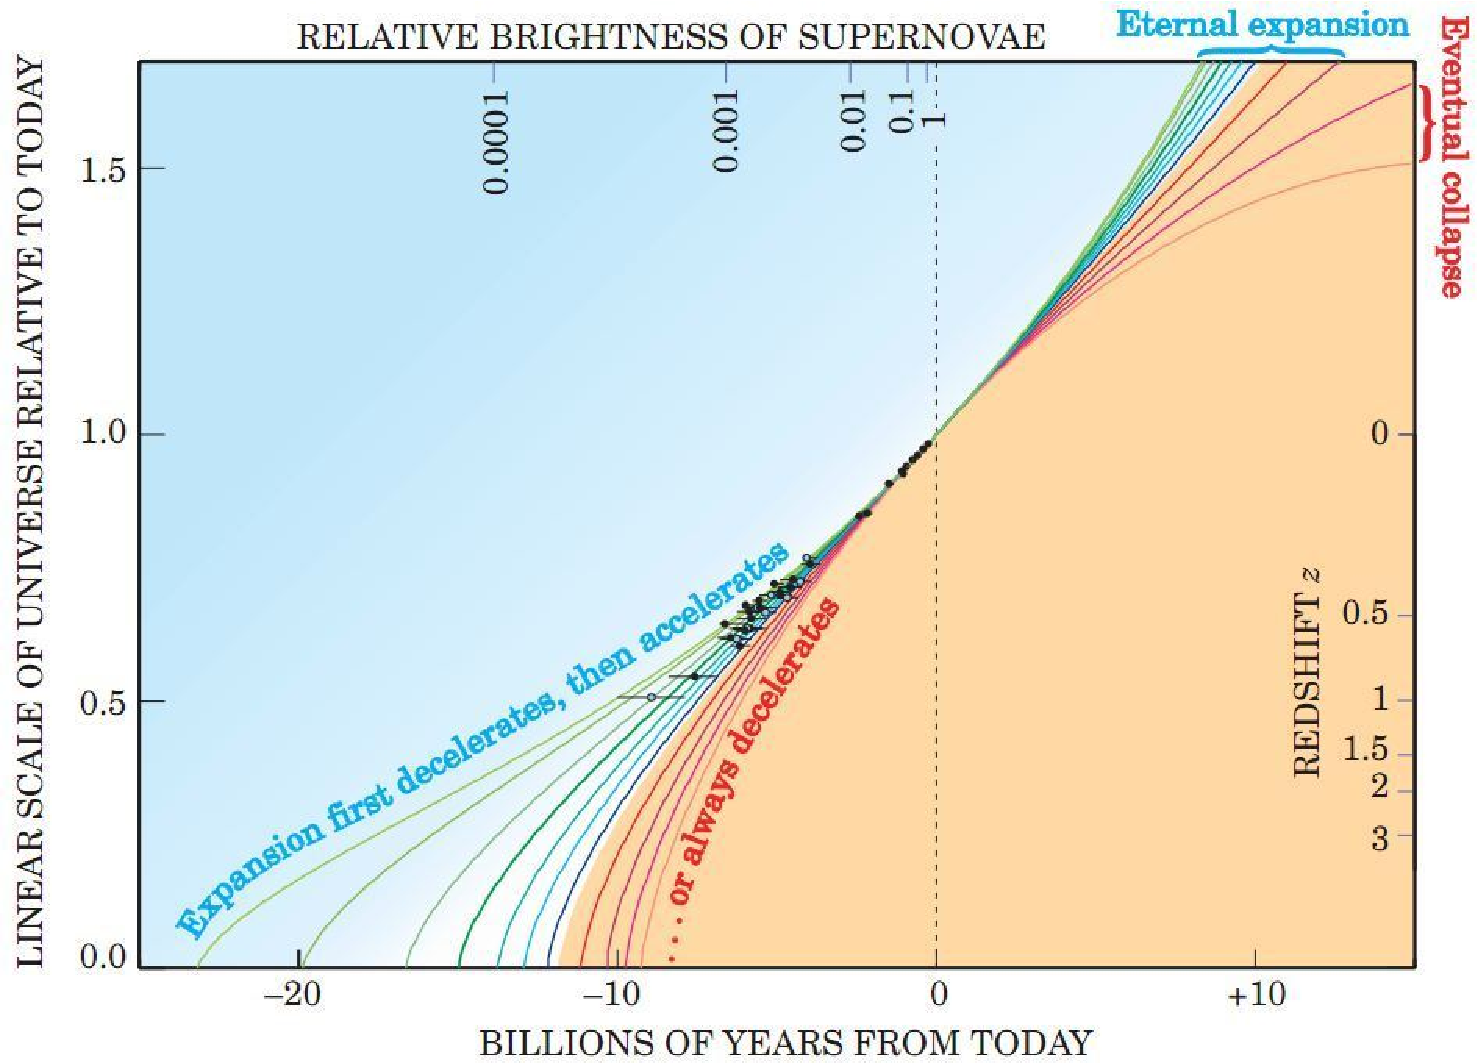
\includegraphics[width=0.8\textwidth]{figure/Scale_Factor_vs-Time.pdf}
  \caption{Andamento $R=R(t)$}
  \label{fig:Rvst}
\end{figure}

Vediamo come sia possibile determinare i parametri di densità $\Omega_i$
attraverso misure di distanza e red-shift.  In effetti, il modo in cui la
costante di Hubble $H(z)$ dipende da $z$ influenza la relazione tra magnitudine
e red-shift.  Preliminarmente osserviamo che dalla definizione $z=R_0/R(t) -1$,
segue
\begin{equation}
  \dd z = -\frac {R_0}{R(t)} H(t) \dd t.
\end{equation}
Consideriamo ora segnali luminosi (per i quali è $d \tau=0$) emessi al tempo $t$
da una galassia che abbia coordinata radiale $r$, e che raggiungono noi (che siamo in
$r=0$) all'istante $t_0$.  Dalla metrica RW si ha
\begin{equation}
  \int_t^{t_0} \frac {\dd t}{R(t)}= \int_0^{r} \frac {\dd r}{\sqrt{1-kr^2}}
  \simeq r + \mathcal{O}(r^3),
\end{equation}
Si ha quindi
\begin{equation}
  r \simeq \int_0^z \frac{\dd z}{R_0 ~ H(t)}.
\end{equation}
La distanza di luminosità $d_L = r R_0 (1+z)$ diventa allora
\begin{equation}
  \begin{split}
    d_L(z) & = (1+z) \int_0^z \frac{\dd z}{H(z)} = \\
           & = (1+z) \int_0^z \frac{\dd z}{H_0
             \left[\Omega_{\Lambda}+\Omega_{k}(1+z)^2+\Omega_m
               (1+z)^3\right]^{1/2}}.
  \end{split}
\end{equation}
Quindi a parità di $z$, gli oggetti osservati (di stessa magnitudine assoluta
$M$) appaiono più o meno lontani a seconda del valore dei parametri cosmologici
(vedere Fig. \ref{fig:Par_Cosm} dove per le supernovae \footnote{In sistemi
  binari di una nana bianca ed una gigante rossa, la massa espulsa dalla gigante
  rossa cade sulla nana bianca, che esplode in supernova quando la sua massa
  supera la massa limite di Chandrasekar. Si ritiene che queste supernovae
  abbiano la stessa luminosità intrinsceca, indipendentemente dalla distanza.}
di tipo Ia (??per la presenza o assenza di particolari righe??) è mostrata la
distanza $d_L$ in funzione del red-shift $z$).  È evidente allora che lo studio
del diagramma $m-z$ per questi oggetti (sufficientemente lontani) permette di
determinare i valori dei parametri $\Omega_{\Lambda}$, $\Omega_{k}$ ed
$\Omega_{m}$.
% In particolare si ha $\Omega_m = 0.27$ ed $\Omega_{\Lambda} =0.73$, se si
% assume $\Omeka_k=0$, il che è dedotto dall'analisi delle anisotropie della
% temperatura della CMB.%


Ricordiamo che per i modelli di Friedmann, la relazione $d_L=d_L(z)$ era
\begin{equation}
  d_L = \frac {1}{H_0} \left[ z+ \frac{1}{2}(1-q_0)z^2\right].
\end{equation}

Questo programma è stato realizzato prendendo come indicatori di distanza le
supernovae di tipo Ia~\parencites{1998AJ....116.1009R}{1999ApJ...517..565P}
\begin{figure}
  \centering
  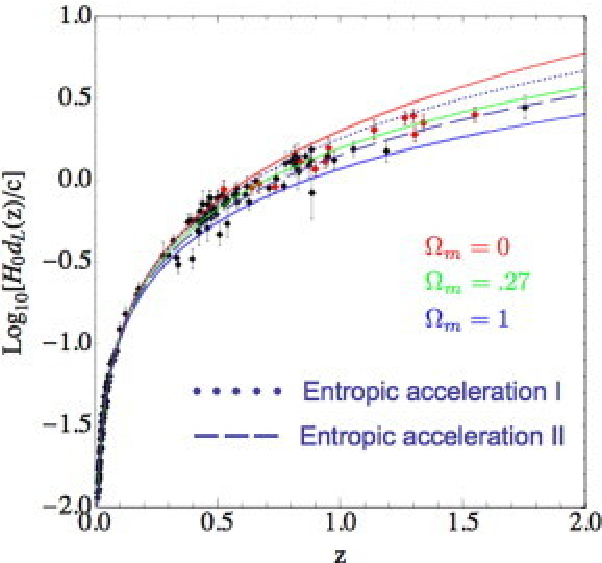
\includegraphics[width=0.8\textwidth]{figure/Hubble_Diagr_1_SNIa.pdf}
  \caption{Diagramma di Hubble SNIa}
  \label{fig:DHSN1}
\end{figure}
% \begin{figure}
%   \centering
%   \includegraphics[scale=1.2]{figure/Hubble_Diagr_2_SNIa.pdf}
%   \caption{Diagramma di Hubble SNIa.}
%   \label{fig:DHSN2}
% \end{figure}
e unitamente all'analisi di dati relativi all'anistrotropia della temperatura
della CMB e della funzione di correlazione angolare di galassie, si sono
determinati i seguenti valori
\begin{subequations}
  \begin{align}
    \Omega_k &= 0, \\
    \Omega_{\Lambda} &\simeq 0.7, \\
    \Omega_{m} &\simeq 0.3.
  \end{align}
\end{subequations}
La figura~\ref{fig:Par_Cosm} mostra che nello spazio dei parametri cosmologici
vi sono tre differenti regioni permesse --- quelle che danno $\chi^2<1$ --- la
cui intersezione determina la regione di valori permessi.
\begin{figure}
  \centering{}
  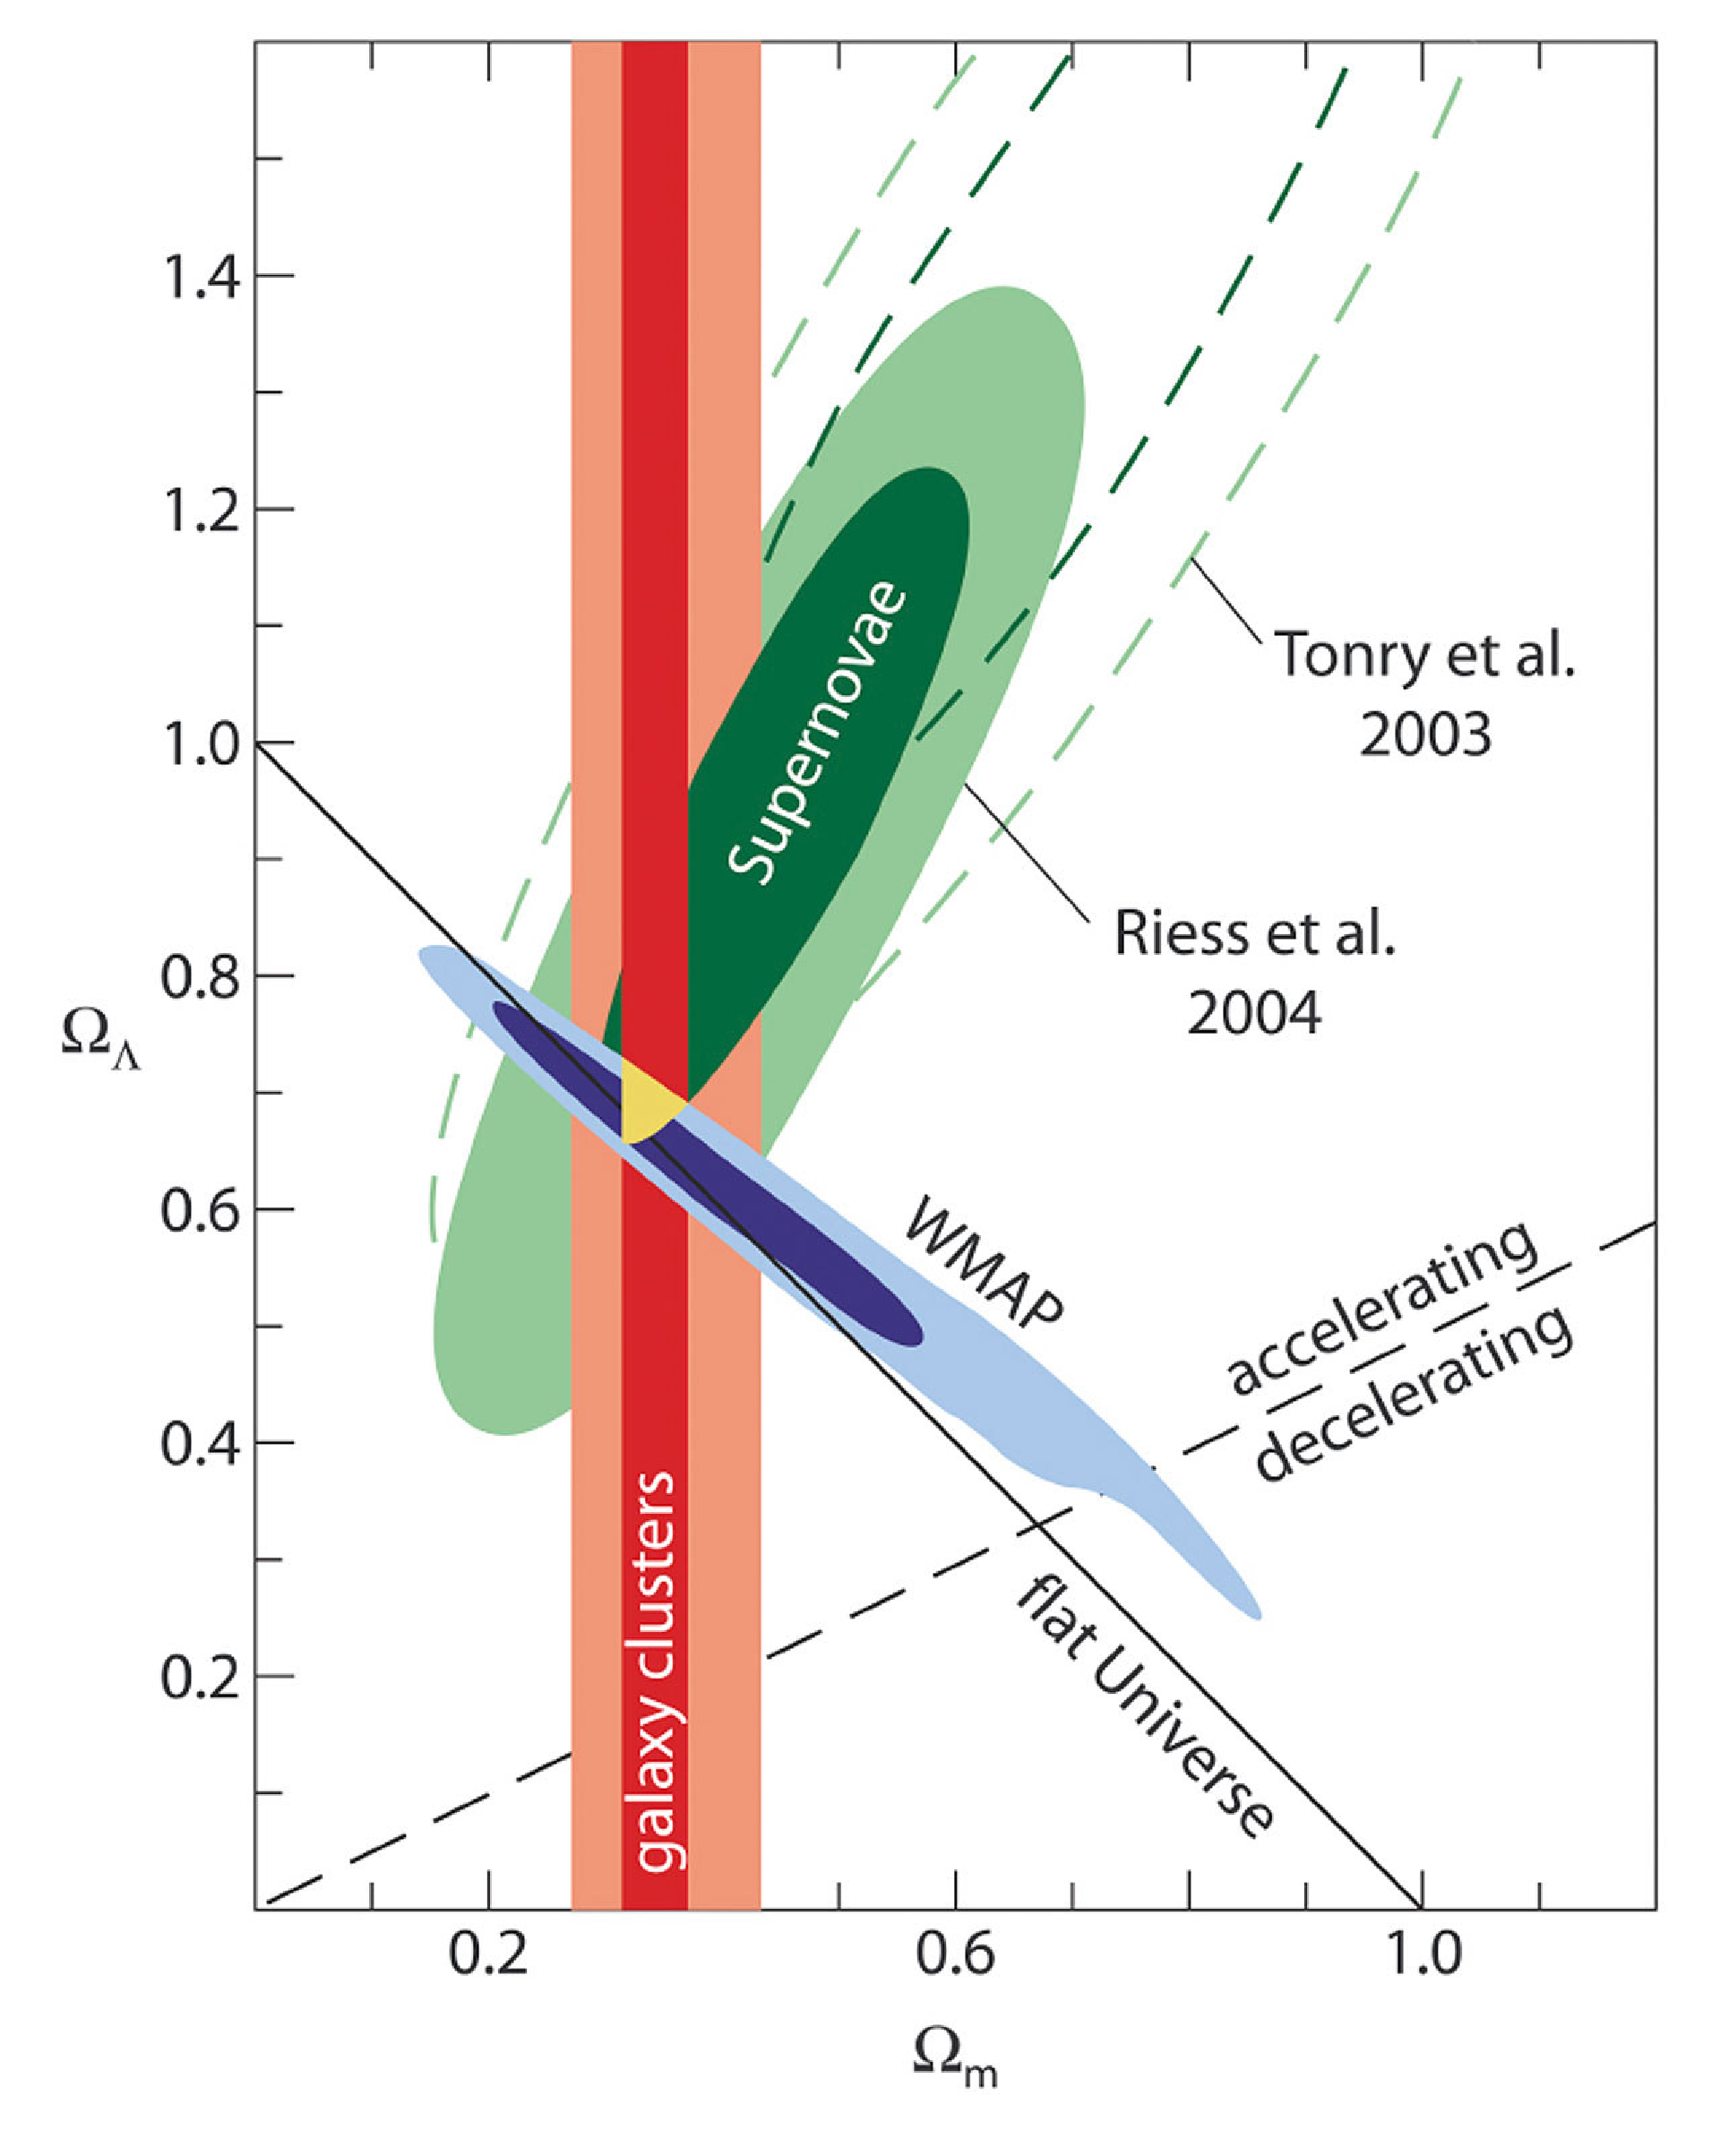
\includegraphics[width=0.6\textwidth]{figure/Cosmological_parameters.pdf}
  \caption{Spazio dei parametri $\Omega_{m}$, $\Omega_{\Lambda}$, $\Omega_k$}
  \label{fig:Par_Cosm}
\end{figure}

\subsubsection{Dark Energy}

Dal punto di vista fenomenologico, invece di introdurre nelle eq. di Einstein (a
sinistra) il termine $g_{\mu \nu}\Lambda$, possiamo introdurre (a destra) un
termine di sorgente con densità $\rho_{DE}$, che attribuiamo ad una nuova
componente dell'Universo nota come Dark Energy.  In generale si assume che la
Dark Energy abbia eq. di stato $p_{DE}=w\rho_{DE}$ con $w<0$.  Il caso $w=-1$
corrispondente alla costante cosmologica.  Ora, se assumiamo che la componente
DE sia disaccoppiata dalla radiazione
\begin{equation}
  \toder{(\rho_{DE} R^3)}{R} = -3 p_{DE} R^2
\end{equation}
si ha
\begin{equation}
  \rho_{DE} \propto \frac {1}{R^{3(1+w)}}
\end{equation}
Pertanto $\rho_{DE}=\text{cost}$ implica $w=-1$ come per il caso
$\rho_{\Lambda}=\text{cost}$, $p_{\Lambda}=-\rho_{\Lambda}$.

Notiamo che il rapporto $\rho_{DE}/\rho_m \propto R^{-3w} \propto (1+z)^{3w}$.
Quindi nel caso $w<0$, per $t < t_0 $ ($z$ crescente a partire dal valore 0), si
ha $\rho_{DE}/\rho_m \to 0$, cioè l'importanza della componente DE diminuisce
indietro nel tempo e i risultati dei modelli di Friedmann non sono modificati
per $z\gg 1$ dalla presenza della componente DE.

L'eq. \eqref{hzcc} risulterà così modificata:
\begin{equation}
  H(z)=H_0 \left[ \Omega_{DE} (1+z)^{3(1+w)} + \Omega_{k} (1+z)^2+ \Omega_m
    (1+z)^3 \right]^{1/2}
  \label{hzccX}
\end{equation}

Anche l'eq. (\ref{ddRcc}) è modificata
\begin{equation}
  \frac {\ddot{R}} {R} = H_0^2
  \left[ - \frac{\Omega_{DE} (1+3w)}{2} (1+z)^{3(1+w)}
    -\frac {\Omega_m (1+z)^3} {2 } \right]
  \label {ddRw}
\end{equation}
da cui per il parametro di decelerazione si ha ora
\begin{equation}
  q_0= \frac{\Omega_{DE}}{2} (1+3w) +  \frac{\Omega_m}{2} + \Omega_{k}
\end{equation}
e, nel caso $k=0$ (poichè $\Omega_m = 1 - \Omega_{DE}$), si ha
\begin{equation}
  q_0= \frac {1+3w \Omega_{DM}}{2},
\end{equation}
per cui se poniamo $\Omega_{DE} \simeq 0.7$ si ha $q_0 =0.5+w$ che diventa
negativo (quindi l'Universo oggi è in una fase di espansione accelerata) se
$w<-0.5$.  In realtà lo studio dei diagramma di Hubble $m-z$ non permette una
precisa determinazione del valore di $w \simeq -0.7$ a causa delle larghe
incertezze dei dati osservativi.

%Tornando indietro alla relazione $d_L(z)$ osserviamo che nel caso $\Omega_{k}=0$
%ed $\Omega_{\Lambda}=0$
%\begin{equation}
%d_L =
%\end{equation}
%mentre se prendo $\Omega_{k}=0$ ed  $\Omega_{m}=0$
%\begin{equation}
%d_L = (1+z) \int_0^z \frac{dz}{H_0 (1+z)^{3(1+w)/2}}
%\end{equation}
%e per $w=-1$ segue $d_L=H_0^{-1} z (1+z)$. Quindi a parità di $z$ oggetti
%appaiono più o meno distanti a seconda del valore dei parametri cosmologici
%$\Omega$.  Vedi figura da cui si ottiene (assumendo $k=0$ $\Omega_{m}=0.32$ ed
%$\Omega_{\Lambda}=0.68$)

L'introduzione della costante cosmologica nelle eq. di Einstein
può essere interpretata in due modi:
\begin{itemize}
\item nel primo caso è come se la lagrangiana della materia sia modificata con
  l'aggiunta di un termine costante
  \begin{equation}
    L_{\textup{matter}} \to L'_{\textup{matter}} = L_{\textup{matter}} -
    \frac{\Lambda}{8 \pi G},
  \end{equation}
  così che l'integrale d'azione diventa
  \begin{equation}
    S_{tot}=S_{g}+S_{m}= \frac {1}{16 \pi G} \int R \sqrt{-g} \dd^4x + \int
    \left( L_{m}- \frac {\Lambda}{8 \pi G} \right) \sqrt{-g} \dd^4 x.
  \end{equation}
  L'eq. del moto per la materia (descritta dal campo $\phi$) che sono ottenute
  variando $S$ rispetto $\phi$ e ponendo $\delta S/\delta \phi=0$, rimangono
  inalterate poiché $\Lambda=\text{cost}$.  In questo caso l'introduzione del
  termine $\Lambda$ introduce solamente uno shift nel livello zero dell'energia
  della materia e non influenza la dinamica della materia, mentre la gravità che
  è accoppiata alla energia totale del sistema ne è influenzata;
\item il secondo caso corrisponde ad un integrale d'azione scritto come
  \begin{equation}
    S_{tot}= \frac {1}{16 \pi G}
    \int (R-2\Lambda)  \sqrt{-g} \dd^4x + \int  L_{m} \sqrt{-g} \dd^4 x,
  \end{equation}
  e la gravità risulta descritta dalle due costanti $G$ e $\Lambda$.  In questo
  secondo caso lo spazio-tempo è curvo anche in assenza di materia.
\end{itemize}

L'eq. di stato $\rho=-p$ ha un'altra importante implicazione in relatività
generale.  La parte spaziale $\bm{g}$ dell'accelerazione geodetica (che misura
l'accelerazione di due particelle di prova molto vicine) soddisfa l'eq.
\begin{equation}
  \nabla \cdot \bm{g} = - 4 \pi G (\rho+3p)~,
\end{equation}
per cui la causa dell'accelerazione geodetica è $\rho+3p$.  Quindi se
$\rho+3p<0$, la gravità diventa repulsiva.

Questo starebbe accadendo oggi nell'Universo poichè all'istante attuale la DE
domina ($\rho_{\Lambda}+3 p_{\Lambda} <0$).  La transizione dalla gravità
attrattiva (dovuta alla materia ordinaria) a quella repulsiva avverrebbe a un
red-shift $\simeq 0.5$.

Quanto vale $\Lambda$?  Preliminarmente osserviamo che $\Lambda$ ha dimensioni
cm$^{-2}$.  La velocità della luce e l'istante attuale $t_0$ definiscono una
lunghezza caratteristica (raggio visibile dell'Universo nel caso $k=1$) $l_0 = c
t_0 \simeq c/H_0 \simeq 10^{28}$ cm $\simeq$3 Gpc.  Poiché l'Universo appare
omogeneo ed isotropo su questa scala (non vi sono effetti indotti da $\Lambda$
nella distribuzione di sorgenti) $\Lambda < 10^{-56}$ cm$^{-2}$.

\section{Radiazione di fondo cosmico}

La radiazione di fondo cosmico nella banda delle microonde (CMB) ha uno spettro
di corpo nero a $T_{CMB}(0) \simeq 2.725$K.  Nella Figura~\ref{fig:radio-gamma}
lo spettro della radiazione extragalactica è mostrato in funzione dell'energia
dei fotoni.  La CMB contribuisce con il 93\% dell'emissione totale.  Definita la
grandezza $f_{\lambda}= \rho_{\lambda}/\rho_{tot}$, si ha:
$f_{CMB}=0.93,$ $f_{IR}= 0.05$, $f_{VIS}=0.02$, $f_{X}=2.5
\times 10^{-4},$ $f_{\gamma}= 2.5 \times 10^{-5}$, $f_{CR} \simeq
\Omega_{CMB}$.
\begin{figure}
  \centering{}
  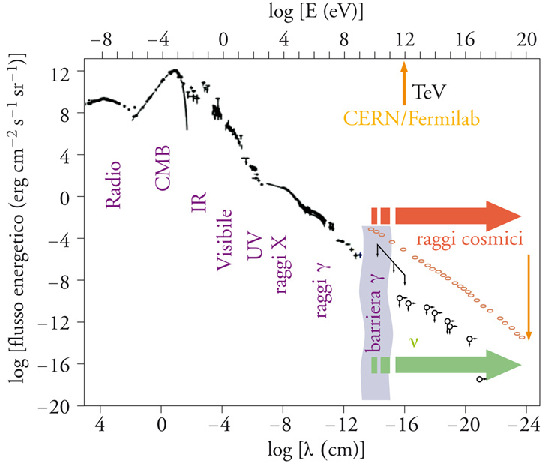
\includegraphics[width=0.8\textwidth]{figure/Radiazione_radio_gamma.pdf}
  \caption{Radiazione dal radio al gamma}
  \label{fig:radio-gamma}
\end{figure}
\begin{figure}
  \centering{}
  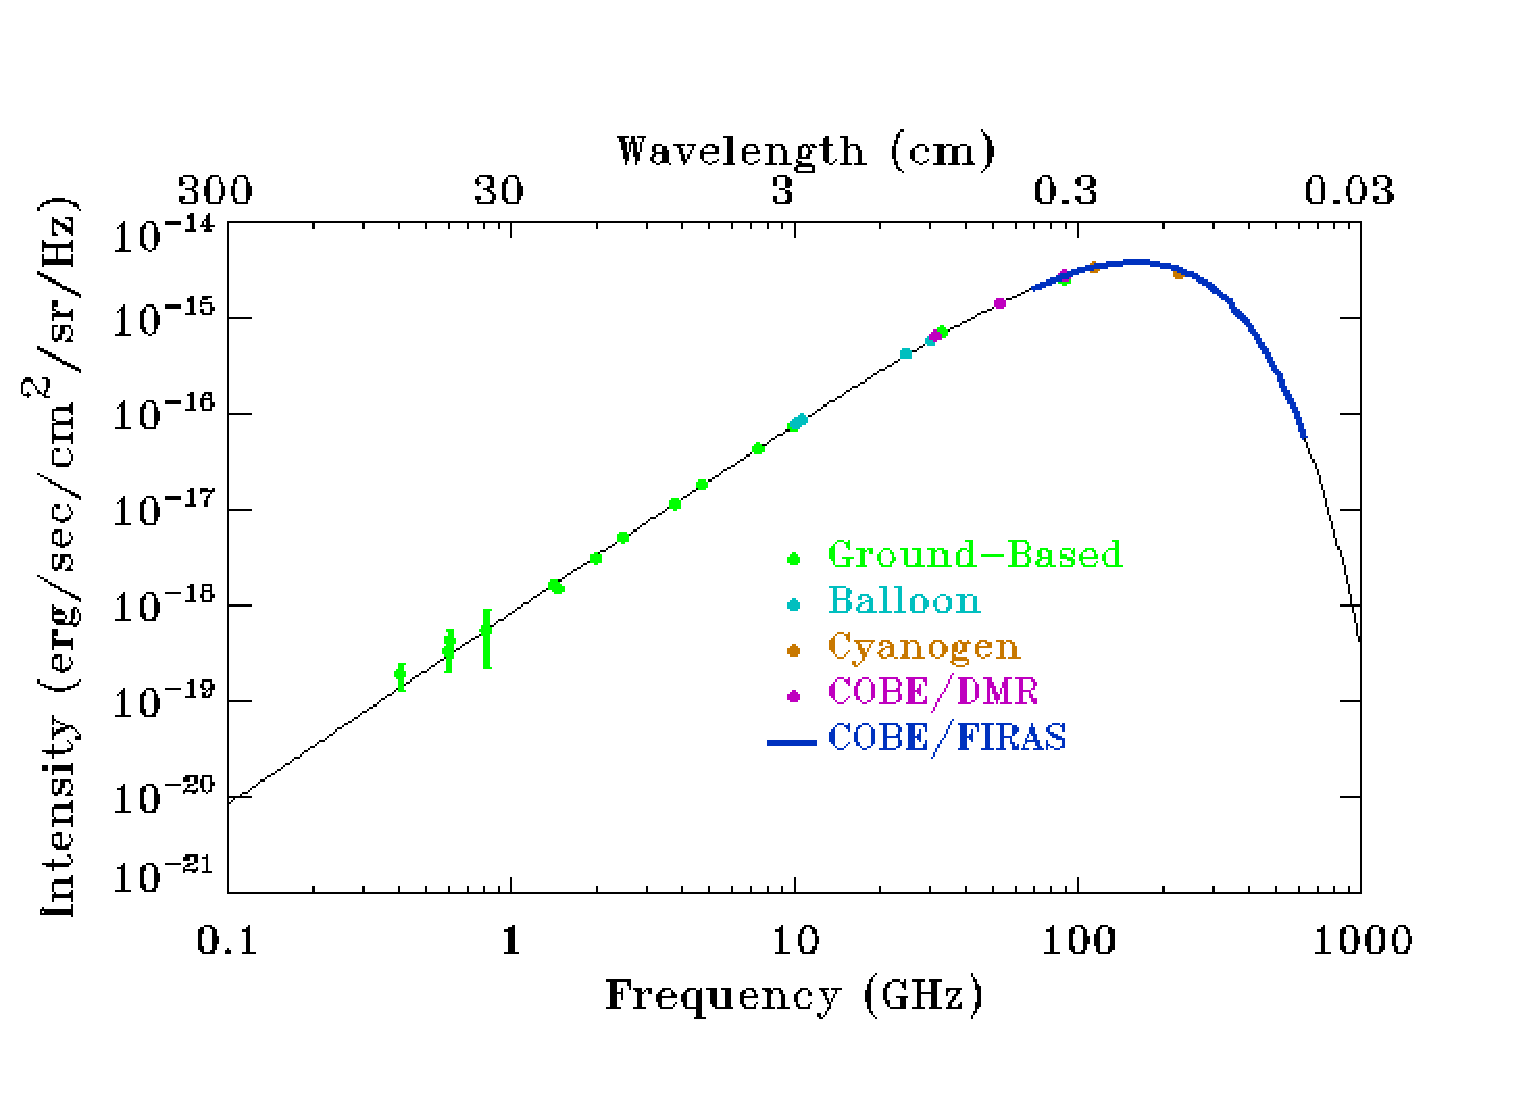
\includegraphics[width=\textwidth]{figure/CMB_intensity.pdf}
  \caption{CMB e distribuzione di Planck a $T_{CMB} = 2.75$K}
  \label{fig:spettro_CMB}
\end{figure}
La densità di energia di un gas di bosoni è
\begin{equation}
  d \rho (p)  = g \frac{4 \pi p^2 dp} {h^3} \frac{1} {\exp[ E(p) / kT ]-1} E(p)
\end{equation}
e poichè (i fotoni sono bosoni di massa nulla) $E(p)=pc=h\nu$ e $g=2$, si ha
\begin{equation}
  d \rho_{\gamma}(\nu) =   \frac{8 \pi h \nu^3 } {c^3} \frac{1} {\exp(h \nu/ kT)
    -1} d\nu
  \label{spettro_BB}
\end{equation}

Posto $x=(h \nu/kT)$, nello spettro di corpo nero si distingue la regione di
Rayleigh-Jeans (con $x\ll 1$) in cui lo spettro cresce come $x^2$ e la regione
di Wien con spettro decrescente come $x^3 \exp(-x)$.  Il massimo dello spettro
si trova derivando l'eq.  \eqref{spettro_BB} rispetto ad $x$ e uguagliando a
zero.  Si ottiene $3(\exp x_{max} -1) = x_{max} \exp(x_{max})$, che ha soluzione
numerica $x_{max} \simeq 2.8$. Quindi $(h \nu_{max}) \simeq 2.8 kT_{max}$, da
cui $(h \nu_{max}) \simeq 2.4 \times 10^{-4}$ eV o, equivalentemente,
$\lambda_{max} \simeq 1.7$ mm, $\nu_{max} \simeq 1.8 \times 10^{11}$ Hz.

La densità totale di energia si calcola integrando lo spettro su tutte le
frequenze
\begin{equation}
  \begin{split}
    \rho_{\gamma}(t_0) &= \int_0^{\infty} \frac{8 \pi h \nu^3 } {c^3}
    \frac{\dd\nu} {\exp (h \nu/
      kT_0) -1} \\
    &= \frac{8 \pi k^4 T^4_0}{c^3 h^3} \int_0^{\infty} \frac{x^3}{e^{x} -1} \dd
    x \\
    & = a T^4_0 \\
    & = 4.64 \times 10^{-34}~~{\rm gr~cm^{-3}} \implies \Omega_{\gamma} =2.47
    \times 10^{-5} h^{-2}
\end{split}
\end{equation}
dove $a=(8 \pi k^4)/(15 h^3 c^3) = 7.56 \times 10^{-15}$ erg cm$^{-3}$
deg$^{-4}$ è la costante di Stefan-Boltzmann, e $h$ è la costante di Hubble in
unità di $100$ km/sec/Mpc, cioè $h=H_0/100$ km/sec/Mpc.

La densità spaziale di fotoni della CMB all'istante attuale è
\begin{equation}
  \begin{split}
    n_{\gamma}(t_0) & = \int_0^{\infty} \frac{\rho_{\gamma}(t_0) } {h \nu }
    \dd\nu
    = \frac{8 \pi k^3 T^3_0 }{c^3 h^3} \int_0^{\infty} \frac{x^2}{e^x -1} \dd x
    \\
    & = \frac{30 a \zeta(3) T^3_0} {\pi^4 k} = 0.3702 \frac{a T^3_0}{k} = 410
    ~{\rm fotoni/cm^3}
  \end{split}
\end{equation}
L'attuale  densità di nucleoni  è invece
\begin{equation}
  n_N (t_0) = \frac{3 \Omega_B H_0^2}{8 \pi G m_N c^2} =
  1.123 \times 10^{-5} \Omega_B h^2 ~{\rm nucleoni/cm^3}
\end{equation}
e il rapporto tra le due densità rimane costante nel tempo (perché entrambe
variano come $\propto R^{-3}$)
\begin{equation}
  \frac{n_{\gamma}(t_0)}{n_N(t_0)} = 3.65 \times 10^{7}.
\end{equation}

A temperature $T>4000~$K l'Universo è opaco alla radiazione con $\gamma$, H$^+$,
e$^-$ in contatto termico alla stessa temperatura e $\gamma$ con spettro di
corpo nero; a $T \simeq 4000$K si forma l'idrogeno neutro e l'Universo diventa
trasparente alla radiazione, nel senso che l'assorbimento di un fotone alla
frequenza $\nu= \Delta E/h$ è seguito da emissione isotropa di un fotone alla
stessa frequenza.

Ma lo spettro continua ad essere di corpo nero. Per dimostrarlo, supponiamo che
la transizione tra Universo opaco e Universo trasparente avvenga istantaneamente
al tempo di ultimo scattering $t_{LS}$ a cui la temperatura ha il valore
$T_{LS}$.

Se consideriamo tempi successivi $t>t_{LS}$ abbiamo le seguenti proprietà
\begin{itemize}
\item fotoni che al tempo $t$ hanno frequenza $\nu$, a $t_{LS}$ avevano
  frequenza (maggiore) $\nu R(t)/R(t_{LS})$
\item a causa dell'espansione la densità propria di fotoni diminuisce come
  $[R(t_{LS})/R(t)]^3$.
\end{itemize}
Quindi, al tempo $t$ la densità di fotoni con frequenza tra $\nu$ e $\nu+d\nu$ è
determinata a partire dalla densità al tempo $t_{LS}$ modificata dalle proprietà
precedenti:
\begin{equation}
  n_{\gamma}(\nu, t) d\nu = \left( \frac {R(t_{LS})} {R(t)} \right)^3
  8 \pi \nu^2 d \nu
  \left( \exp \left[ \frac {h} {k T_{LS}} \frac{\nu R(t)}{R(t_{LS})} \right] -1
  \right)^{-1} \left( \frac {R(t)} {R(t_{LS})} \right)^3
\end{equation}
da ciò si vede che $n_{\gamma}(\nu,t)$ è una distribuzione di corpo nero a ogni
$t$ se
\begin{equation}
  T(t) = T_{LS} \frac {R(t_{LS})} {R(t)}
\end{equation}

Questa conclusione è inalterata se la transizione dall'opacità alla trasparenza
avviene in un tempo finito poichè l'interazione $\gamma H$ è limitata allo
scattering elastico per il quale le frequenze dei $\gamma$ non cambiano.

Dopo il disaccoppiamento tra materia e radiazione si ha $\rho_{\gamma} \propto
R^{-4}$ e poiché $\rho_{\gamma} \propto T^4$, si ha $T_{\gamma} \propto
R(t)^{-1}$.  Ma prima del disaccoppiamento come varia la temperatura dei fotoni
in contatto termico con la materia?  A questo scopo consideriamo un semplice
modello per l'Universo che supponiamo costituito da un gas ideale e radiazione
alla stessa temperatura $T_{\gamma}=T_{m}=T$. Densità e pressione delle due
componenti sono
\begin{subequations}
  \begin{align}
    \rho_{\gamma} & = a T^4 \\
    p_{\gamma} &=\rho/3  \\
    \rho_{m}    & = n_N m c^2 + \frac{p_{m}}{\gamma-1} \\
    p_m &=n_N kT
  \end{align}
\end{subequations}
dove l'indice politropico $\gamma=5/3$ $(4/3)$ per il regime non relativistico
(relativistico).  Per la densità e pressione totali avremo $\rho =
\rho_{m}+\rho_{\gamma}$ e $p=p_{m}+p_{\gamma}$ e sostituendo
nell'eq. \eqref{moto} si trova l'eq. differenziale
\begin{equation}
  \label{TvsR}
  \frac{R}{T} \toder{T}{R} = -
  \left(\frac{\sigma+1}{\sigma+[3(\gamma-1)]^{-1}}\right)
\end{equation}
dove la costante $\sigma = 4 a T^3_{\gamma}/(3 n_N k)$ è l'entropia specifica.  Ora:
\begin{itemize}
\item se $\sigma \ll 1$, dall'eq. \eqref{TvsR} segue $T \propto
  R^{-3(\gamma-1)}$ che è l'usuale relazione temperatura-volume per
  un'espansione adiabatica di un gas ideale, e infine
  $T \propto R^{-1}$ nel caso relativistico (per cui $\gamma=4/3$)
e $ T \propto R^{-2}$ nel caso non-relativistico (per cui $\gamma=5/3$);
\item se $\sigma \gg 1$ si ha sempre $T \propto R^{-1}$.
\end{itemize}

Nel nostro caso $\sigma = 4 a T^3_{\gamma}(0)/(4 n_N(0) k) \simeq 10^8$ e quindi
prima del disaccoppiamento la materia (nonostante sia in un regime
non-relativistico) segue la radiazione con $T_m=T_{CMB} \propto R^{-1}$.  Dopo
il disaccoppiamento la temperatura della materia $T_{m}\propto R^{-2}$.

\subsection{Anisotropia di dipolo}

Supponiamo che vi sia un sistema di riferimento fondamentale in cui la
radiazione di fondo cosmico sia isotropa (e con spettro di Planck) e che la
Terra si muova con velocità $v_{\oplus}$ rispetto a questo sistema.  Nel sistema
fondamentale, i fotoni nell'angolo solido $\sin \theta \dd \theta \dd \phi$ e
con frequenza tra $\nu$ e $\nu + \dd\nu$ contribuiscono al tensore energia
impulso della radiazione di fondo cosmico con
\begin{equation}
  \dd T^{\mu \nu}=  \left( \frac{p^{\mu} p^{\nu}}{h^2 \nu^2} \right)
                  \left( \frac{\sin\theta \dd\theta \dd\phi}{4\pi} \right)
  \rho_{\gamma 0}(\nu) \dd\nu
\label{521}
\end{equation}
Nella relazione precedente si è tenuto conto che il tensore energia impulso è
proporzionale a $p^{\mu} p^{\nu}$ (vedi~\cite[44]{weinberg:gravitation}); gli
altri termini sono introdotti in modo che integrando sull'intero angolo solido
$\dd T^{00} = \rho_{\gamma 0} \dd \nu$.  Si ha quindi
\begin{equation}
  \dd T^{\mu \nu}= \left( 2 \frac{ p^{\mu} p^{\nu} }{h} \right)
                   \left( \frac{1} { \exp (h \nu/ kT_{\gamma 0 }) } \right)
  \sin \theta \dd\theta \dd\phi \nu \dd\nu
\label{522}
\end{equation}
con
\begin{equation}
  p^{\mu} \equiv (E, p_x, p_y, p_z) =
  h \nu ( 1, \sin \theta \cos \phi , \sin \theta \sin \phi, \cos \theta)
\end{equation}

Nel sistema della Terra il tensore energia impulso della radiazione di fondo è
\begin{equation}
  \dd T'^{\mu \nu} = \tensor{\Lambda}{^{\mu}_{\rho}} \tensor{\Lambda}{^{\nu}_{\sigma}}
  \dd T^{\rho\sigma}
\end{equation}
dove $\Lambda$ è la matrice di Lorentz con $\vec{v} = - \vec{v}_{\oplus}$.
Allora possiamo esprimere $\dd T'^{\mu \nu}$ in termini di quantità nel sistema
della Terra.  Osserviamo preliminarmente
\begin{equation}
  p'^{\mu } = \tensor{\Lambda}{^{\mu}_{\nu}} p^{\nu}
\end{equation}
e che orientando gli assi in modo ($\phi=0$) che l'asse z sia nella direzione della
velocità della Terra,  si ha
\begin{subequations}
  \begin{gather}
    \nu' = \nu \frac{[1-v_{\oplus}\cos\theta]}{[ 1 - v_{\oplus}^2]^{1/2}}, \\
    \cos\theta' = \frac{[- v_{\oplus} + \cos\theta]}{[1 - v_{\oplus}
      \cos\theta]}, \\
    \phi' = \phi
  \end{gather}
\end{subequations}
dove ora $\theta$ è l'angolo tra la velocità della Terra e il fotone.
Il tensore energia impulso differenziale nel sistema terra ha necessariamente la forma
\begin{equation}
  \dd T^{\prime \mu \nu}= \left( 2 \frac{ p^{\prime \mu} p^{\prime \nu} }{h} \right)
                   \left( \frac{1} { \exp (h \nu/ kT_{\gamma 0 }) } \right)
  \sin \theta \dd\theta \dd\phi \nu \dd\nu
\end{equation}
poich\'e in eq.(\ref{522}) il termine a sinistra \'e un tensore di rango 2 controvariante,
il prodotto $p^{\mu} p^{\nu}$ \'e un tensore dello stesso tipo e rango e quindi la parte
restante a destra \'e un invariante.
Ora, l'angolo solido ha la regola di trasformazione (?)
\begin{equation}
 \sin \theta^{\prime} \dd\theta^{\prime} \dd\phi^{\prime}
= \left( \frac {\nu}{\nu^{\prime}} \right)^2 \sin \theta \dd\theta \dd\phi
\end{equation}
da cui segue
\begin{equation}
  \dd T^{\prime \mu \nu}= \left( 2 \frac{ p^{\prime \mu} p^{\prime \nu} }{h} \right)
                   \left( \frac{1} { \exp (h \nu^{\prime}/ kT^{\prime}_{\gamma 0 }) } \right)
  \sin \theta^{\prime} \dd\theta^{\prime} \dd\phi^{\prime} \nu^{\prime} \dd\nu^{\prime}
\end{equation}
dove si \'e posto
\begin{equation}
T^{\prime}_{\gamma 0} \equiv \left( \frac{\nu ^{\prime}}{\nu} \right) T_{\gamma 0} =
\left[ \frac{(1- v_{\oplus} \cos \theta)}{(1-v_{\oplus}^2)^{1/2} } \right] T_{\gamma 0}
\end{equation}
Quindi, rispetto alla Terra la radiazione di fondo cosmico ha ancora una distribuzione di Planck
ma con una temperatura differente.
Per velocit\'a piccole, cio\'e per $v_{\oplus}/c << 1$, segue che
\begin{equation}
\Delta T_{\gamma 0} = T^{\prime}_{\gamma 0} - T_{\gamma 0} = - \frac{ v_{\oplus}} {c} T_{\gamma 0}
\end{equation}
Questa relazione determina un'anisopropia di dipolo in due direzioni opposte.
Da misure recenti si trova $v_{\oplus} \simeq 300$ km/s (nel direzione ....) e quindi
$  \Delta T_{\gamma 0} / T_{\gamma 0} \simeq 10^{-3}$.

\subsection{Effetto GZK}

I raggi cosmici, prevalentemente protoni, sono prodotti da acceleratori cosmici
(SN galattiche fino ad energia $E_{CR} \simeq 10^{15}$ eV, AGN extragalattici
per energie maggiori) ed hanno uno spettro che si estende da circa $10^9$ ev fino a $10^{21}$ ev
seguendo semplici leggi di potenza. (Vedi Fig. \ref{fig:CR1})
 \begin{figure}
   \centering{}
   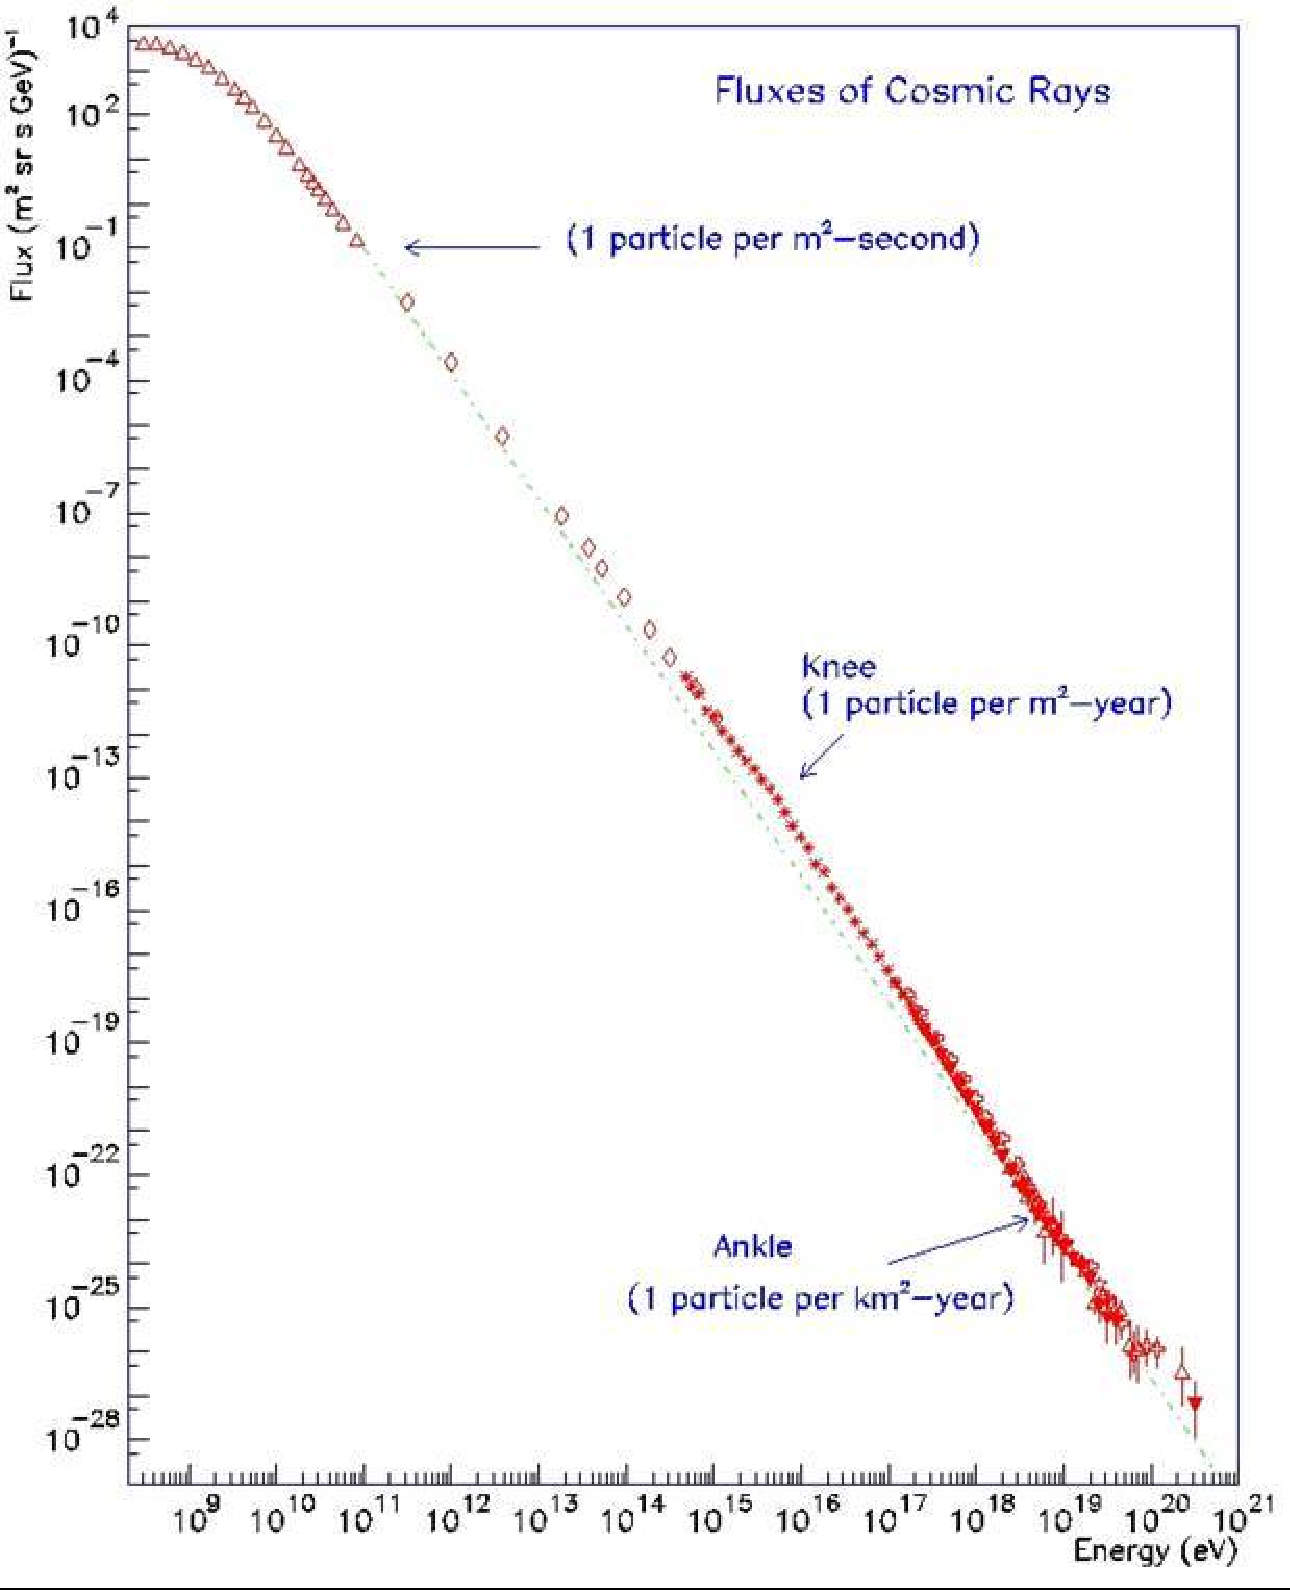
\includegraphics[width=0.8\textwidth]{figure/CR_spectrum_1.pdf}
  \caption{Spettro dei Raggi Cosmici}
  \label{fig:CR1}
\end{figure}
Comunque ad energie $E_{CR} \simeq 10^{20}$ eV si osserva nello spettro dei CR
una perdita di flusso che è una dimostrazione indiretta dell'esistenza della
CMB: protoni di alta energia interagiscono con i fotoni del fondo cosmico dando
luogo ad interazioni forti del tipo $p \gamma_{CMB} \to p \pi^0$ e $\gamma_{CMB}
p \to n \pi^+$, e quindi non ci raggiungono.  Tali processi, comunque, avvengono
attraverso la creazione di risonanze (stati metastabili intermedi)
$\Delta^{++}$, $\Delta^{+}$, $\Delta^{0}$ e il loro successivo decadimento.
L'effetto è stato predetto
da~\textcites{1966PhRvL..16..748G}{1966JETPL...4...78Z}.

La massa della risonanza $m_{\Delta} \simeq 1236$ MeV pone un limite inferiore
all'energia dei protoni dei CR capaci di attivare il processo di annichilazione.
Consideriamo la cinematica del processo.  Nel sistema del laboratorio sia
\begin{subequations}
  \begin{align}
    P^{\mu}_{\gamma}       &= (q, \bm{q}), \\
    P^{\mu}_{\ \textup{p}}   &= (\sqrt{p^2+m^2_\textup{p}}, \bm{p}), \\
    P^{\mu}_{\ \textup{tot}} &= ( q+\sqrt{p^2+m^2_\textup{p}}  ,  \bm{q} + \bm{p}) \\
    \sqrt{s} &= \sqrt{ P^{\mu}_{\ \textup{tot}} P_{\mu \ \textup{tot}} } =
                        \left[ \left( q+\sqrt{p^2+m^2_\textup{p}} \right)^2 -
                        \left(\bm{q}+ \bm{p} \right)^2 \right]^{1/2} \\
                      & \simeq \left[ 2qp \left(1-\cos \theta \right) +
                        m_\textup{p}^2 \right]^{1/2}.
  \end{align}
\end{subequations}
La reazione può avvenire se $\sqrt{s} > m_{\Delta} c^2$.  La tipica energia
$\langle E_{\gamma}\rangle$ dei fotoni della CMB è $6 \times 10^{-4}$ eV e il
massimo di $(1-\cos \theta)=2$.  Si ha quindi
\begin{equation}
  p_{\textup{th}} \simeq \frac{m^2_{\ \Delta} c^4 - m^2_{\ p} c^4} {4 \langle
    \ E_{\gamma}\rangle} \simeq 10^{20}~~~{\rm eV}
\end{equation}
Nella figura~\ref{fig:CR2} è riportato lo spettro dei raggi cosmici attorno al
taglio GZK.
\begin{figure}
  \centering{}
  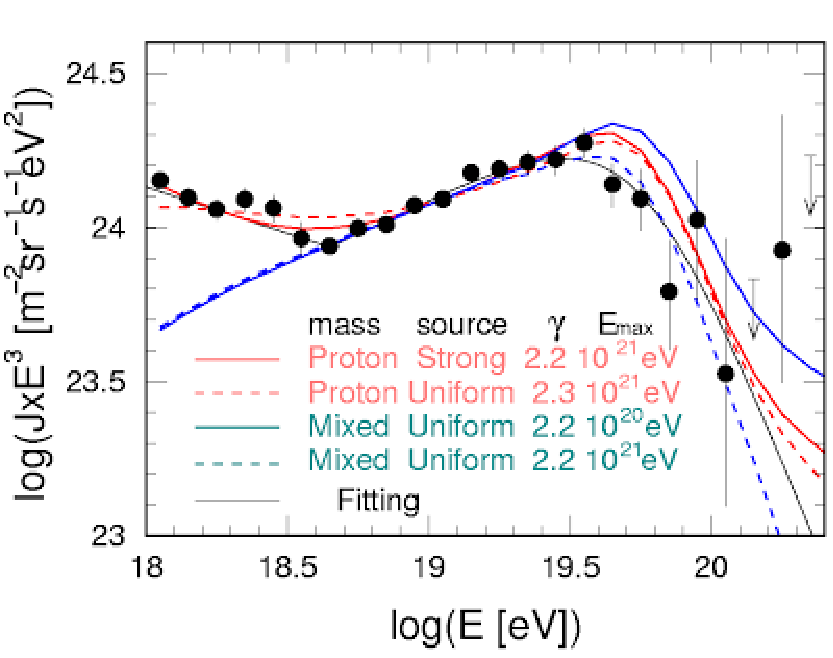
\includegraphics[width=\textwidth]{figure/CR_spectrum_2.pdf}
  \caption{Spettro dei Raggi Cosmici a $E \simeq 10^{20}$ eV}
  \label{fig:CR2}
\end{figure}

\section{Conservazione dell'entropia}

Si consideri un gas perfetto con densità e pressione $\rho= \rho(T)$ e $p=p(T)$.
Le leggi della termodinamica sono
\begin{subequations}
  \label{leggi_termo}
  \begin{align}
    \dd Q &= \dd U+p\dd V \\
    \dd S &= \frac{\dd Q}{T}
  \end{align}
\end{subequations}
in cui $dQ$ è il calore assorbito, $dU=d(\rho c^2 V)$ la variazione di energia
interna, $pdV$ il lavoro eseguito, $dS$ la variazione di entropia, $V$ infine è
il volume occupato dal gas.

Dalle leggi della termodinamica si ha
\begin{equation}
  \begin{split}
    \dd S &=  \frac{1}{T} \left( \dd( \rho c^2 V) + p \dd V \right) \\
    &= \frac{1}{T} \left( V \dd(\rho c^2) + (\rho c^2+p) \dd V \right) \\
    &= \frac{1}{T} \left( V \toder{(\rho c^2)}{T} \dd T + (\rho c^2+p) \dd V
    \right).
  \end{split}
\end{equation}
Poichè $S=S(V,T)$ segue
\begin{equation}
  \dd S = \left( \frac{\partial S}{\partial T} \right)_V \dd T +
  \left( \parder{S}{V} \right)_T \dd V
\end{equation}
dal confronto tra le precedenti eq. si ha
\begin{subequations}
  \begin{align}
    \left(\parder{S}{V}\right)_T &= \frac{1}{T} (\rho c^2+p) \\
    \left(\parder{S}{T}\right)_V &= \frac{V}{T} \toder{(\rho c^2)}{T}.
  \end{align}
\end{subequations}
La condizione di integrabilità
\begin{equation}
  \frac{\partial}{\partial T} \left( \frac{\partial S}{\partial V} \right) =
  \frac{\partial}{\partial V} \left( \frac{\partial S}{\partial T} \right)
\end{equation}
conduce alla relazione
\begin{equation}
  \toder{p}{T} = \frac{1}{T} (\rho c^2 +p).
  \label{integrab}
\end{equation}
Usando questa relazione nella legge di conservazione dell'energia \eqref{moto}
si ha
\begin{equation}
  \begin{split}
    \toder{}{t} [R^3(\rho c^2 +p)] & = R^3 \toder{p}{t} \\
    & = R^3 \toder{p}{T} \toder{T}{t} \\
    & = R^3 (\rho c^2 +p) \frac{1}{T} \toder{T}{t}
  \end{split}
\end{equation}
da cui segue
\begin{equation}
  \toder{}{t} \left( \frac{R^3}{T} (\rho c^2 + p) \right) = 0.
\end{equation}
Se indichiamo con $S(t)$ l'entropia contenuta nel volume comoving, abbiamo
\begin{subequations}
  \begin{align}
    S(t) & =  \left( \frac{R^3}{T} (\rho c^2 + p) \right) \\
    \toder{S(t)}{t} & = 0 \iff S(t)= \text{cost}
  \end{align}
  \label{cons_entropia}
\end{subequations}
che esprime la conservazione dell'entropia contenuta in un volume comoving (che
scala come $R^3$).

Verifichiamo che la definizione di $S$ è consistente con la $2^a$ legge della
termodinamica in eq. \eqref{leggi_termo}, che riscriviamo nella forma
\begin{equation}
  \dd S  = \frac{1}{T} \left( \dd(\rho c^2 V) + \dd(pV) - V \toder{p}{T} dT
  \right)
\end{equation}
e usando l'eq. \eqref{integrab}
\begin{equation}
  \begin{split}
    \dd S &= \frac{1}{T} \left( \dd(\rho c^2 V + pV) -  \frac{V}{T}   (\rho c^2
      +p) \dd T \right) \\
    &= \dd\left( \frac{V (\rho c^2 + p)} {T}  \right)
  \end{split}
\end{equation}
che è la relazione in eq. \eqref{cons_entropia} poiché $V \propto R^3$.

\section{Universo primordiale}

Si prende ora in esame l'era dell'Universo dominata dalla radiazione, per cui
\begin{equation}
  \rho(t)=\rho_0 \left(\frac{R_0}{R(t)} \right)^4
  \label{293}
\end{equation}
La dinamica dell'Universo è descritta dall'eq. \eqref{eq:friedmann}, in cui ora
però si può trascurare il termine $k$
\begin{equation}
  \dot{R}^2 = \frac{8 \pi G}{3} \rho R^2,
  \label{fri_pri}
\end{equation}
in quanto il termine $(8 \pi G /3) \rho R^2$ risulta essere $\gg 1$ nell'era
della radiazione.  Infatti, all'istante attuale $t_0$ si ha
\begin{equation}
  \frac{8 \pi G}{3} \rho_0 R^2_0 = \frac{2q_0}{|2q_0-1|} > 0.03
\end{equation}
poichè $q_0>0.014$.  D'altra parte indietro nel tempo, tale termine cresce
almeno come $z$ e quando $z\simeq 1000$ (inizio era radiazione) risulta $>30$.

Da eq. \eqref{293} e \eqref{fri_pri} si ha
\begin{equation}
  \frac{\dot \rho}{\rho} = -4 \frac{\dot R}{R} = - 4 \left( \frac{8 \pi G
      \rho}{3} \right)^{1/2}
\end{equation}
da cui segue la relazione tra $t$ e $\rho$
\begin{equation}
  t = \left( \frac{3}{32 \pi G \rho} \right)^{1/2} + \text{cost}\ .
  \label{tvsrho}
\end{equation}

L'obiettivo ora è quello di ricavare $\rho= \rho(T)$.  Ovviamente ci riferiamo
ad un era in cui le galassie non si erano ancora formate ed il fluido
cosmologico è diffuso con densità (quasi) uniforme.  In realtà all'interno della
materia (prevalentemente dark) e della radiazione sono presenti (i semi delle
galassie) le fluttuazioni di densità (prodotte da transizioni di fase tra
$10^{-43} - 10^{30} sec$, durante l'epoca inflazionaria) che si accrescono a
causa del meccanismo di Jeans (instabilità gravitazionali di sistemi di
dimensioni maggiori della lunghezza d'onda di Jeans).  Al disaccoppiamento,
comunque, i contrasti di densità sono ancora molto piccoli, poiché $\Delta \rho
/ \rho \simeq \Delta T / T \simeq 10^{-5}$ durante l'era in cui ci è contatto
termico tra materia e radiazione. I picchi di densità successivamente si
accrescono fino alla creazione di strutture autogravitanti di materia oscura. Si
formano quindi prima sistemi autogravitanti di materia oscura e poi su queste
buche di potenziale gravitazionale cadono i barioni, che attraverso processi
dissipativi, alla fine danno luogo alle strutture visibili ammassi, galassie,
stelle.

A partire dal tempo a cui le interazioni deboli ed elettromagnetiche si sono separate,
$t > 10^{-30}$ secondi, $T < 100 $ Gev, i costituenti dell'Universo vanno ricercati
tra le seguenti particelle:
\begin{itemize}
\item gli adroni = barioni (n,p,..) \& mesoni ($\pi$, k, ...) e rispettive
  antiparticelle;
\item i leptoni = e, $\mu$, $\tau$, $\nu_e$, $\nu_{\mu}$, $\nu_{\tau}$ e
  rispettive antiparticelle;
\item i fotoni,
\end{itemize}
e la composizione del fluido cosmologico ad ogni $T(t)$ è caratterizzata da:
\begin{itemize}
\item particelle di massa $m$ in equilibrio con la radiazione, con $mc^2\ll kT$;
\item particelle di massa $m$ disaccoppiate dalla radiazione, con $mc^2\gg kT$;
\item particelle in transizione con $mc^2 \simeq kT$.
\end{itemize}
Nel primo caso la temperatura dei fotoni è sufficientemente alta così che le
reazioni di creazione e di annichilazione
\begin{equation}
  \text{particella + antiparticella} \to \gamma \gamma
\end{equation}
procedono con la stessa rate nei due sensi.

Nel secondo caso, la temperatura è bassa (rispetto alla massa a riposo) e le
reazioni avvengono prevalentemente nel verso dell'annichilazione, il che produce
rapidamente la scomparsa delle antiparticelle (si ipotizza che l'Universo nasca
con un eccesso di particelle) lasciando alla fine tracce di particelle.


Con riferimento alle masse delle particelle e alla relazione $m c^2 = kT$, si
definisce una scala di temperatura (K$^{-1} = 11604$ Kelvin/eV):
\begin{table}
  \centering{}
  \caption{Corrispondenza $m c^2 = kT$}
  \label{massa_temp}
  \begin{tabular}{ccc}
    \toprule
    T (deg)         & Energia    & T (K)              \\
    \midrule
    $m_n c^2$       & 939.55 MeV & $1.090 \times 10^{13}$ \\
    $m_p c^2 $      & 938.25 MeV & $1.088 \times 10^{13}$ \\
    $m_{\tau}c^2$   & 177    MeV & $2.1   \times 10^{12}$ \\
    $m_{\pi} c^2$   & 140    MeV & $1.6   \times 10^{12}$ \\
    $m_{\mu} c^2 $  & 106    MeV & $1.2   \times 10^{12}$ \\
    $(m_n-m_p) c^2$ & 1.3    MeV & $1.5   \times 10^{10}$ \\
    $m_e c^2      $ & 511    KeV & $5.8   \times 10^{9 }$ \\
    temperatura di dissociazione del deuterio \\
    \bottomrule
  \end{tabular}
\end{table}
in cui si distinguono le seguenti fasi:
\begin{itemize}
\item[(A)] $T \gg 10^{13}$K: tutte le particelle presenti (era adronica);
\item[(B)] $T \simeq 10^{12}$K: gli adroni sono scomparsi; rimangono tracce di
  adroni (n,p) in eccesso rispetto alle antiparticelle inizialmente presenti, e
  tutti leptoni;
\item[(C)] $T < 10^{12}$K: i leptoni pesanti $\mu$ e $\tau$ scompaiono e i
  neutrini $\nu_e$, $\nu_{\mu}$ e $\nu_{\tau}$ disaccoppiano con temperatura
  $T_{\nu}$; il fluido cosmologico è composto da n, p, e$^-$, e$^+$, $\gamma$ in
  equilibrio alla stessa temperatura $T$;
\item[(D)] $T < 10^{11}$K: la differenza di massa tra neutroni e protoni produce
  un eccesso di protoni;
\item[(E)] $T < 5 \times 10^{9}$K: ($t \simeq $ 4 sec dalla singolarità), le
  coppie $\text{e}^- \text{e}^+ \to \gamma \gamma$, lasciando tracce di p, n,
  e$^-$, $\gamma$ in equilibrio ad una temperatura $T > T_{\nu}$ dei neutrini
  già disaccoppiati;
\item[(F)] $T \simeq 10^{9}$K: ($t \simeq 180$ sec) i nuclei di deuterio
  diventano stabili e i neutroni sopravvissuti al decadimento in protoni
  rapidamente si fondono nei nuclei degli elementi leggeri; da questo momento
  fino alla ricombinazione l'Universo è costituito da un plasma ionizzato,
  prevalentemente $H^+$, $^4He^2$ ed elettroni (nella percentuale di 1 atomo di elio per
  ogni 11 atomi di idrogeno), in equilibrio con i $\gamma$, mentre i neutrini
  già disaccoppiati sono a temperatura più bassa;
\item[(G)] tra $(4000 < T < 10^{9})$K: espansione libera con $T_m = T \propto
  R^{-1}$ e $\gamma$ termalizzati (con spettro di corpo nero) fino alla
  ricombinazione;
\item[(H)] tra $(10^3 -10^5)$K, l'Universo entra nell'era della materia.
\end{itemize}

Ricorrendo ai metodi della meccanica statistica è possibile ora esprimere le
densità di energia delle particelle presenti nell'Universo alle varie epoche in
funzione della temperatura.  Infatti, nell'approssimazione di gas perfetto,
fermioni e bosoni sono descritti dalle statistiche di Fermi-Dirac e
Bose-Einstein. Per la specie $i$, la densità in numero di particelle con impulso
tra $q$ e $q+dq$ è
\begin{equation}
  n_i(q) \dd p = \frac{g_i 4 \pi q^2 \dd q} {h^3} \left( \exp\left[{
        {\frac{E(q)-\mu_i}{KT}} }\right] \pm 1 \right)^{-1}
\end{equation}
in cui l'energia $E =(q^2+m^2)^{1/2}$, $\mu_i$ è il potenziale chimico, il segno
$+$ per fermioni, il segno $-$ per bosoni, $g_i$ la molteplicità rispetto allo
spin ($g_i=2 s_i+1$ per particelle di massa $m_i \ne 0$, $g_i=2$ per fotoni e
neutrini).

Con la semplificazione $\mu_i=0$ (particelle e antiparticelle uguali in numero)
ed $E \simeq q$ (tutti i leptoni sono relativistici) si ha:
\begin{subequations}
  \begin{align}
    \rho_{\gamma} & = a T^4 \\
    \rho_e &=\rho_{\mu}=\rho_{\tau} = \frac{7}{8} a T^4 \\
    \rho_{\nu}    & = \frac{7}{16} a T^4.
  \end{align}
\end{subequations}
Queste relazioni permettono di esprimere $\rho$ ad ogni epoca in funzione di $T$
(trascurando le tracce di barioni).

Nell'intervallo di temperatura $(10^{10} < T < 10^{12})$K la densità totale del
fluido cosmologico è
\begin{equation}
  \rho = 2 \left(\rho_{\nu_\textup{e}} + \rho_{\nu_{\mu}} + \rho_{\nu_{\tau}} +
    \rho_{\textup{e}} \right)+\rho_{\gamma}=\frac{43}{8}a T^4
\end{equation}
con neutrini disaccoppiati dal fluido e $T_{\nu}=T$.  Quando la temperatura
$T<10^{10}$K, ma prima dell'annichilazione delle coppie e$^+$ e$^-$, l'entropia
del fluido cosmologico (elettroni, positroni, fotoni e tracce di nucleoni) è
\begin{equation}
  S_{\textup{prima}}= \frac{R^3}{T} (\rho c^2 +p) = \frac{11}{3} a (RT)^3
\end{equation}
mentre per $T<5 \times 10^9$K (dopo l'annichilazione delle coppie e$^{-}$ e$^+$)
sono presenti solamente fotoni con tracce di nucleoni ed elettroni; allora
\begin{equation}
  S_{\textup{dopo}}= \frac{4}{3}\frac{R^3}{T} \rho_{\gamma} = \frac{4}{3} a (RT)^3
\end{equation}
Poichè $S_{\textup{prima}} = S_{\textup{dopo}}$ (entropia nel volume comoving è
costante), ci deve essere un brusco salto della temperatura dei fotoni (di cui
non risente la componente dei neutrini già disaccoppiati).  Man mano che
l'Universo si espande la temperatura delle due componenti, fondo cosmico e di
neutrini, diminuisce come $R^{-1}$ ed oggi vi sono due fondi di radiazione a
temperatura diversa
\begin{equation}
  T_{\nu}(t_0) = \left(\frac{4}{11}\right)^{4/11} T_{CMB}(t_0)
\end{equation}

Per $T<10^9$K la densità di energia della radiazione (fotoni e neutrini) è data
da $\rho_r \simeq 1.45 a T^4$.  Questo valore di densità deve essere confrontato
con la densità della materia $\rho_m(t) \simeq n_N(t) m_N c^2$ che invece scala
come $R^{-3}$ (la materia è in un regime non relativistico).  Esisterà allora
una temperatura critica $T_{\textup{crit}}$ a cui le densità si uguagliano,
$\rho_r(T_{\textup{crit}}) = \rho_m (T_{\textup{crit}})$ e al di sotto della
quale, l'Universo diventa dominato dalla materia.  Tale valore di temperatura
dipende da $n_N(t_0)$
\begin{equation}
  T_{crit} \simeq 4200\text{K} \left( \frac {m_N n_N(0)}{10^{-30}~{\rm gr~ cm}^{-3}} \right)
\end{equation}
e per valori di $m_N n_N(0)$ nel range $(2 \times 10^{-29} - 3 \times 10^{-31})$
gr cm$^{-3}$ risulta nel range di valori $(1200 < T_c < 84.000)$K.

Infine, a $T_R \simeq 4000$K si forma l'idrogeno neutro, la CMB si disaccoppia
dalla materia e si propaga fino a noi, mantenendo ``l'imprinting della
\emph{superficie di ultimo scattering}''.  Quanto tempo trascorre dalla
singolarità al disaccoppiamento?  Dalla relazione~\eqref{tvsrho} si ha che
partendo da $T=10^{12}$K passano 0.01 sec perché la temperatura cada a
$10^{11}$K e altri 1.07 sec perché $T=10^{10}$K.  Alla fine della sintesi degli
elementi sono trascorsi 180 sec; il disaccoppiamento tra materia e radiazione
avviene a circa 400.000 anni.  (Vedi la tabella~\ref{storia_termica},
da~\textcite[550]{weinberg:gravitation}.)
\begin{table}
  \centering{}
  \caption{Storia termica dell'Universo a partire dall'annichilazione $\mu+ \mu^-$)}
  \label{storia_termica}
  \begin{tabular}{cccc}
    \toprule
    T (K)               & $R/R_0$               & $T/T_{\nu}$ & t(sec)                \\
    \midrule
    $10^{12}  $         & $1.9 \times 10^{-12}$ & 1.000       & 0                     \\
    $10^{11}  $         & $1.9 \times 10^{-11}$ & 1.000       & 0.01                  \\
    $3 \times  10^{10}$ & $6.4 \times 10^{-11}$ & 1.001       & 0.121                 \\
    $10^{10}   $        & $1.9 \times 10^{-10}$ & 1.008       & 1.103                 \\
    $3  \times 10^{9}$  & $5.9 \times 10^{-10}$ & 1.081       & 13.83                 \\
    $1  \times 10^{9}$  & $2.6 \times 10^{-9}$  & 1.346       & 182                   \\
    $1  \times 10^{8}$  & $2.7 \times 10^{-9}$  & 1.401       & $1.92 \times 10^4$    \\
    $1  \times 10^{6}$  & $2.7 \times 10^{-6}$  & 1.401       & $1.92 \times 10^8$    \\
    $1  \times 10^{4}$  & $2.7 \times 10^{-4}$  & 1.401       & $1.92 \times 10^{12}$ \\
    $4 \times 10^{3}$   & $6.3 \times 10^{-4}$  & 1.401       & $1.20 \times 10^{13}$ \\
    \bottomrule
  \end{tabular}
\end{table}

\section{Sistesi dell'elio}

Gli elementi più abbondanti oggi nell'Universo sono l'idrogeno neutro H e l'elio
$^4$He (2n+2p), presenti nella percentuale di 1 atomo di elio per ogni 11 atomi
di idrogeno; insieme costituiscono $\simeq 99$\% di tutti gli elementi, la
restante parte, con numero atomico $A>4$, sono i metalli (l'abbondanza in
metalli è indicata con $Z$).  L'abbondanza in massa in $^4$He viene indicata con
$Y= m_{^4He}/m_{Totale} = 4 m_N/(4 m_N + 11 m_N) \simeq 0.25$.

Una possibile spiegazione per la presenza di $^4$He è la nucleosintesi nel core
delle stelle.  La teoria, sviluppata da Bethe intorno al 1938, spiega l'energia
emessa dalle stelle attraverso reazioni di fusione termonucleare in cui elementi
leggeri si fondono in elementi più pesanti (ma con massa totale minore della
massa degli elementi di partenza).  Ad esempio nel caso del sole le reazioni più
importanti sono (ciclo pp)
\begin{subequations}
  \begin{align}
    p + n      & \leftrightarrow ^2H + \gamma \\
    ^2H + ^2H  & \leftrightarrow ^3He + n \leftrightarrow ^3H + p \\
    ^3H + ^2H  & \leftrightarrow ^4He + n
  \end{align}
  \label{ciclopp}
\end{subequations}

Le stelle sono però bruciatori troppo lenti per spiegare l'abbondanza osservata.
Infatti, la fusione di 4 protoni in un nucleo $^4$He comporta un rilascio di
energia nelle stelle di 27 Mev, che è emessa prevalentemente in $\gamma$.  Ora,
poiché la massa di un atomo di $^4$He è pari a 3728 Mev$/c^2$, se tutto l'elio
fosse sintetizzato nelle stelle
\begin{equation}
  \frac{\rho_r}{\rho_{He}} > 27/3728 \simeq 0.007
\end{equation}
in cui il simbolo "maggiore di" indica che nell'Universo ci potrebbe essere
radiazione elettromagnetica di origine diversa.  Poiché oggi si osserva $Y
\simeq 0.25$, si ha
\begin{equation}
  \rho_{He} \simeq 0.25 \rho_G
\end{equation}
dove con $\rho_G$ abbiamo indicato la densità di massa delle galassie, o la
densità di massa dei barioni.  Dalle ultime due eq. segue
\begin{equation}
  \frac{\rho_r} {\rho_G} > 0.002
\end{equation}
Quindi se prendiamo $\rho_G \simeq \rho_* \simeq 10^{-31}$ gr cm$^{-3}$,
dovremmo avere
\begin{equation}
  \rho_r > 2 \times 10^{-34}~{\rm gr~ cm}^{-3}
\end{equation}
Dalle osservazioni si determina la densità di energia della radiazione a
differenti lunghezze d'onda.  Dall'esame della Tab. \ref{tab_den_rad_bande}
concludiamo che non più del 10\% dell'elio presente nell'Universo può avere
origine stellare.
\begin{table}
  \centering{}
  \caption{Densità di energia della radiazione in diverse bande}
  \label{tab_den_rad_bande}
  \begin{tabular}{cc}
    \toprule
    banda            & densità di energia {\rm (gr cm$^{-3}$)} \\
    \midrule
    radio             &  $\simeq          10^{-40} $  \\
    microonde (2.7 K) &  $     4.4 \times 10^{-34} $  \\
    visibile          &  $                10^{-35} $  \\
    X-ray             &  $                10^{-37} $  \\
    $\gamma$-ray      &  $                10^{-38} $  \\
    \bottomrule
  \end{tabular}
\end{table}
Il problema della Nucleosintesi trova soluzione in Cosmologia.  Per $t>1$ sec e
$t<200$ sec dalla singolarità iniziale, la temperatura nell'Universo è nel range
$(10^{10}-5 \times 10^{9})$K, cioè nella scala delle energie $\simeq$ MeV dei
processi nucleari.

Il calcolo dell'abbondanza di $^4He$ procede in due passaggi:
\begin{itemize}
\item per primo si calcola il rapporto $n/(n+p)$ tenendo conto dei processi (di
  interazione debole) che alterano il numero di neutroni e protoni a partire da
  $n/(n+p)=0.5$.  Questi sono
  \begin{subequations}
    \label{w1571}
    \begin{align}
      n + \nu  & \longleftrightarrow p  + e^-             \\
      n + e^+  & \longleftrightarrow p +        {\bar\nu} \\
      n        & \longleftrightarrow p + e^-  + {\bar\nu}
    \end{align}
  \end{subequations}
\item quindi si considerano le reazioni che portano alla formazione dell'elio.
\end{itemize}

Le velocità con cui procedono le reazioni \eqref{w1571} sono date
in~\textcite{weinberg:gravitation}; esse dipendono da $T_{\nu}$, $T$ e dal
parametro $Q$ che è la differenza di massa tra $n$ e $p$
\begin{equation}
  Q= m_n c^2 - m_p c^2 \simeq 1.293 {\rm Mev}
\end{equation}
In particolare, a causa della differenza di massa tra $n$ e $p$ le reazioni
procedono con velocità maggiore nel verso della diminuzione del numero di
neutroni.  Le velocià totali sono ($\lambda$ ha dimensioni sec$^{-1}$) (vedi
Winberg)
\begin{subequations}
  \begin{gather}
    \lambda (n \to p) = \lambda (n + \nu \to p + e^-) + \lambda (n + e^+ \to p +
    {\bar \nu}) + \lambda (n \to p + e^- +{\bar \nu }) \\
    \lambda (p \to n) = \lambda (p + e^- \to n + \nu ) + \lambda (p + {\bar \nu}
    \to n + e^+ + \lambda (p + e^- +{\bar \nu} \to n)
  \end{gather}
\end{subequations}
L'eq. differenziale per il rapporto $X_n= n/(n+p)$ è
\begin{equation}
  -\toder{X_n}{t} =  \lambda (n \to p) X_n + \lambda (p \to n) (1-X_n)
\end{equation}
con soluzione numerica data in~\textcite[549]{weinberg:gravitation} e riportata
nella tabella~\ref{X_nvsT}
\begin{table}
  \centering{}
  \caption{Rapporto $X_n=n/(n+p)$ in funzione della temperatura e del tempo}
  \label{X_nvsT}
  \begin{tabular}{ccc}
    \toprule
    T (deg)            & t (sec)    & $X_n$ \\
    \midrule
    $10^{12} $           & 0         & 0.496 \\
    $10^{11}  $          & 0.01      & 0.462 \\
    $3 \times  10^{10}$  & 0.121     & 0.380 \\
    $10^{10}   $         & 1.103     & 0.241 \\
    $1  \times 10^{9}$   &  13.83    & 0.170 \\
    $3  \times 10^{9}$   &  182      & 0.137 \\
    $1  \times 10^{8}$   &  18700    & $10^{-8}$ \\
    \bottomrule
  \end{tabular}
\end{table}
A grandi linee:
\begin{itemize}
\item per $T>10^{10}$K, si ha $T_{\nu}=T$ e $\lambda(p\to n)/\lambda(n\to p)
  \simeq \exp(-Q/kT)$.  Questa dipendenza conduce alla soluzione $X_n \simeq
  [1+\exp (Q/kT)]^{-1}$, per cui partendo da $X_n \simeq 0.5$ a $T= 10^{12}$K si
  ha $X_n=0.38$ quando $T= 3 \times 10^{10}$K.  In questo primo periodo è la
  differenza di massa $Q$ che gioca un ruolo maggiore e tra le reazioni
  \eqref{w1571} le prime due sono le più importanti;
\item per $T<1.4 \times 10^{9}$K, la sola reazione efficace è la terza delle
  \eqref{w1571}) in cui $\lambda \simeq 1013$ sec$^{-1}$, così che
  $X_n(t) \simeq X_n(T=1.4 \times 10^{9}\text{K}) \times  \exp(-t/1013)$. \\
\end{itemize}
Quindi, se non ci fossero le reazioni di sintesi tutti i neutroni decadrebbero
in protoni entro un tempo $\simeq 2 \times 1013$ sec.  Invece a temperature di
circa $10^9$K si avviano le reazioni di nucleosintesi, che procedono molto
velocemente, così che tutti i neutroni ancora presenti a questo tempo sono
velocemente sintetizzati in nuclei di $^4$He
\begin{equation}
  Y = X_{He^4} \text{(dopo la nucl.)} \simeq 2X_n \text{(quando la nucl. si
    avvia)}
\end{equation}
Secondo calcoli dettagliati la temperatura di avvio della nucleosintesi
$T_{Nucl}$ dipende dalla densità di nucleoni presenti.  Con riferimento alla
densità attuale si ha
\begin{itemize}
\item $T_{Nucl} \simeq 0.9 \times 10^9~^0K$ se $\rho_N(0) = 7 \times 10^{-31}$
  gr cm$^{-3}$
\item $T_{Nucl} \simeq 1.1 \times 10^9~^0K$ se $\rho_N(0) = 2 \times 10^{-29}$
  gr cm$^{-3}$.
\end{itemize}
All'aumentare di $\rho_N(0)$ l'Universo si espande più velocemente, e quindi
\begin{itemize}
\item meno tempo intercorre per una diminuzione di temperatura;
\item meno tempo per arrivare all'avvio delle reazioni di nucleosintesi;
\item più neutroni sopravvivono al decadimento.
\end{itemize}

Nella Tab. \ref{tab_abbondanze}~\parencite[555]{weinberg:gravitation} sono
riportate le abbondanze degli elementi leggeri con $A<4$.
\begin{table}
  \centering{}
  \caption{Abbondanze cosmologiche di $^4$He e D in funzione di $\rho_N(t_0)$}
  \label{tab_abbondanze}
  \begin{tabular}{cccccc}
    \toprule
           &                     &                     & $\rho_N(t_0)$ (g/cm$^{3}$) &                      &              \\
    \midrule
           & $10^{-31}         $ & $ 10^{-30}        $ & $3.1\times 10^{-29}$       & $ 10^{-29}         $ & $10^{-28}$   \\
    \midrule
    D      & $6.2\times 10^{-4}$ & $2.3\times 10^{-5}$ & $2.7\times 10^{-7} $       & $2.5\times 10^{-12}$ & $ <10^{-12}$ \\
    He$^4$ & 0.236               & 0.263               & 0.272                      & 0.281                & 0.299        \\
    \bottomrule
  \end{tabular}
\end{table}
Si trova che $Y$ dipende poco da $\rho_N(t_0)$ ed è l'abbondanza osservata per
il deuterio ($\simeq 2 \times 10^{-5}$) che pone un limite superiore
$\rho_N(t_0) \simeq 6 \times 10^{-31}$ gr cm$^{-3}$ --- corrispondente a
$\Omega_B <0.05$ --- alla densità attuale di barioni. Vedi anche la
Fig. \ref{fig:abbondanza}
\begin{figure}
  \centering{}
  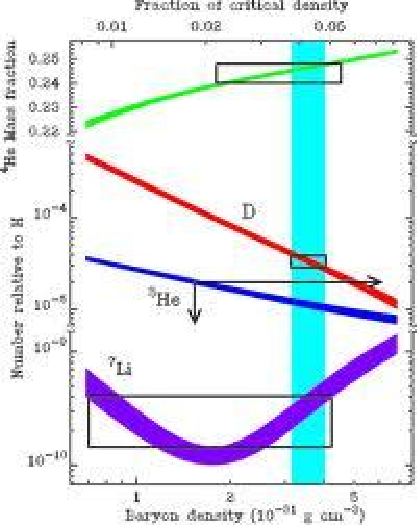
\includegraphics[width=0.5\textwidth]{figure/Abundances.pdf}
  \caption{Abbondanza vs $\rho_B(t_0)$}
  \label{fig:abbondanza}
\end{figure}

%%% Local Variables:
%%% mode: latex
%%% TeX-master: "../cosmo"
%%% fill-column: 80
%%% End:
